\documentclass{as-preprint-template}

\usepackage{amsmath,amsfonts}
\usepackage[english]{babel}
\usepackage[nameinlink,capitalise]{cleveref}
\crefname{equation}{Constraint}{Constraints}

% Tikz
\usepackage{tikz}
\usepackage{pgfplots}
\usepackage{xifthen}
\pgfplotsset{compat=1.13}

% Subfigures
\usepackage{caption}
\usepackage{subcaption}

% Bibliography management
\usepackage[sort,numbers]{natbib}
\bibliographystyle{abbrvnat}

% Tables
\usepackage{booktabs}
\usepackage{rotating}

% Shrinking with resizebox
\usepackage{graphics}

% In-paragraph enumeration
\usepackage{paralist}

\newcommand{\Nat}{\mathbb{N}}
\newcommand{\Rea}{\mathbb{R}}

\newcommand{\itref}[1]{(\ref{#1})}
\newcommand{\keywords}[1]{\vspace{2em}\begin{center}\textbf{Keywords}\end{center}#1}
\newcommand{\contribution}[1]{\vspace{2em}\begin{center}\textbf{Contribution / Potential Impact}\end{center}#1}
\newcommand{\highlights}[1]{\vspace{2em}\begin{center}\textbf{Highlights}\end{center}#1}

\newcommand{\NetGraph}{G_\textup{N}}
\newcommand{\STGraph}{G_\textup{TS}}
\newcommand{\Trains}{I}
\newcommand{\Detours}{D}
\newcommand{\Nodes}{V}
\newcommand{\Arcs}{A}
\newcommand{\STNodes}{V_\textup{TS}}
\newcommand{\STArcs}{A_\textup{TS}}
\newcommand{\Dependencies}{F}

\newcommand{\train}{i}
\newcommand{\trainn}{j}
\newcommand{\trainpath}{p}
\newcommand{\detour}{d}
\newcommand{\node}{v}
\newcommand{\stnode}{w}
\newcommand{\arc}{a}
\newcommand{\timeinstant}{t}
\newcommand{\timestep}{s}
\newcommand{\timethreshold}{\tau}
\newcommand{\dependency}{f}

\newcommand{\softcapacity}{Q}
\newcommand{\hardcapacity}{\overline{Q}}
\newcommand{\arccapacity}{Q}
\newcommand{\canovertake}{\omega}
\newcommand{\mintraveltime}{m}
\newcommand{\maxtraveltime}{M}
\newcommand{\headway}{h}
\newcommand{\dependencytype}{\varepsilon}
\newcommand{\mandatory}{\eta}
\newcommand{\minrestime}{\varphi}
\newcommand{\maxrestime}{\Phi}
\newcommand{\waittime}{w}

\newcommand{\intime}{\theta^\textup{in}}
\newcommand{\outtime}{\theta^\textup{out}}
\newcommand{\minintime}{t^\textup{in}}
\newcommand{\minouttime}{t^\textup{out}}
\newcommand{\maxintime}{T^\textup{in}}
\newcommand{\maxouttime}{T^\textup{out}}

\newcommand{\indelaypenalty}{\pi^\textup{ind}}
\newcommand{\outdelaypenalty}{\pi^\textup{outd}}
\newcommand{\dependencypenalty}{\pi^\textup{dep}}
\newcommand{\capacitypenalty}{\pi^\textup{cap}}
\newcommand{\detourpenalty}{\pi^\textup{det}}

\newcommand{\nbstruct}{\mathcal{N}}
\newcommand{\minmove}{\mu_\textup{min}}
\newcommand{\maxmove}{\mu_\textup{max}}

\newcommand{\rmrk}{\textsuperscript{\textdagger}}

\newcommand{\Instances}{\mathcal{I}}
\newcommand{\Sortings}{\mathcal{S}}
\newcommand{\instance}{i}
\newcommand{\sorting}{s}

\newcommand{\resource}{r}
\newcommand{\uresource}{\rho}
\newcommand{\duresource}{\tilde{\rho}}
\newcommand{\reslength}{l}
\newcommand{\stime}{\lambda_\textup{s}}
\newcommand{\etime}{\lambda_\textup{e}}
\newcommand{\deptime}{\delta}
\newcommand{\source}{\sigma_\textup{src}}
\newcommand{\sink}{\sigma_\textup{snk}}
\newcommand{\sstnode}{\stnode_\textup{s}}
\newcommand{\estnode}{\stnode_\textup{e}}


\setTitle{A Real-Time Conflict Solution Algorithm for the Train Rescheduling Problem}
\addAuthor{Andrea}{Bettinelli}{Optit s.r.l., Italy\thanks{andrea.bettinelli@optit.it}}
\addAuthor{Alberto}{Santini}{Universitat Pompeu Fabra, Spain\thanks{alberto.santini@upf.edu}}
\addAuthor{Daniele}{Vigo}{Università di Bologna, Italy\thanks{daniele.vigo@unibo.it}}
\setJournal{Transportation Research Part B: Methodological}
\setPages{237--265}
\setVolume{106}
\setYear{2017}
\setDoi{10.1016/j.trb.2017.10.005}
\setUrl{https://www.sciencedirect.com/science/article/pii/S0191261516301151}

\begin{document}
  \printCover{}
  \newpage{}
  \maketitle{}

  \abstract{%
    We consider the real-time resolution of conflicts arising in real-world train management applications. In particular, given a nominal timetable for a set of trains and a set of modifications due to delays or other resources unavailability, we are aiming at defining a set of actions which must be implemented to grant safety, e.g., to avoid potential conflicts such as train collisions or headway violations, and restore quality by reducing the delays. To be compatible with real-time management, the required actions must be determined in a few seconds, hence specialized fast heuristics must be used.

    We propose a fast and effective parallel algorithm that is based on an iterated greedy scheduling of trains on a time-space network. The algorithm uses several sortings to define the initial train dispatching rule and different shaking methods between iterations. The performance is further enhanced by using various sparsification methods for the time-space network. The best algorithm configuration is determined through extensive experiments, conducted on a set of instances derived from real-world networks and instances from the literature. The resulting heuristic proved able to consistently resolve the existing conflicts and obtaining excellent solution quality within just two seconds of computing time on a standard personal computer, for instances involving up to 151 trains and two hours of planning time horizon.
  }

  \section{Introduction}\label{sec:introduction}

Modern railways represent a major form of transport with an ever-growing user base, as trains are flexible in terms of travelling distance (they can be used for local, regional and long-distance services) and capacity (as they are modular by nature). Furthermore, train transportation is usually the greenest transportation options for both goods and people.

Despite this, railways are confronted with the increase of operational costs and a fierce competition from other modes of transport. Many users demand more reliability in train operations: a long delay, a cancelled train, a missed connection can easily decrease the perceived quality of service and turn away potential customers.

Most of the events that negatively affect train operations (broadly called \emph{conflicts}) happen when, for some reason, there is a difference between the nominal and the actual service. The causes of such events are usually divided into \emph{disturbances} and \emph{disruptions} (\citet{Cacchiani2014}). The former are small perturbations of the system that are handled by network operators by momentarily changing the timetable. The results of disturbances are usually minor, such as one or more delayed trains, or a platform change at a station. Disruptions, on the other hand, are major incidents that not only alter the nominal timetable, but also require changes in rolling stock and crews. The outcome of a disruption could include major delays, train cancellations, and long reroutings. Disturbances clearly happen much more often than disruptions and their impact is not to be underestimated: a train that is delayed just a few minutes can make a user miss an important connection and increase their travel time by hours. In this paper we consider both disturbances and disruptions in a unified way, by defining an algorithmics approach to handle the conflicts they cause.

Increasing systemwide reliability is crucial at every phase of the planning process. It starts at the strategic and tactical levels (budget allocation for maintenance, timetable robustness, etc.), but once at the operational level, it is almost impossible to avoid that day-to-day activities be disturbed by many kinds of unforeseen events.

When such an event occurs, it is the job of the \emph{dispatcher} to restore the system in a working state. The job of dispatchers has been traditionally done by hand, based exclusively on their experience and practice. It was not until recent years that computer algorithms were developed with the aim of aiding the dispatchers in making the best decision that resolves the critical situation and minimises deviances from the nominal timetable.

In this paper we present such an algorithm, developed to solve the Train Rescheduling Problem (TRP): given a nominal timetable which has become infeasible because of one or more \emph{conflicts} that have arisen, we are asked to produce a new conflict-free timetable that is as close as possible to the nominal one. Or, in case it is not possible to produce a conflict-free timetable, we need to warn the dispatcher about this and provide a timetable with the least possible number of conflicts.

Conflicts are all those situations that either can't physically happen (e.g., two trains occupying the same segment of track at the same time) or that can potentially compromise the safety of operations in the network (e.g., two trains running too close to each other in the same direction).

The algorithm presented in this paper is the result of a long lasting collaboration with Alstom, initiated by the company in 2012 with the aim of redesigning the optimisation algorithms incorporated in its Train Management System ICONIS. To this end, Alstom involved three important Italian research groups in specific research projects investigating various optimisation problems arising in the real time conflict resolution. As a result of such initial wide research effort, the team formed by Optit, an accredited spinoff of the University of Bologna, and the Department of Electrical, Electronic and Information Engineering of the University of Bologna, was selected to produce an innovative real-time conflict solution algorithm capable of taking into account the characteristics and constraints of practical applications which has been developed and industrialised during 2013, and extensively tested by Alstom in real-world contexts. Recently, the new algorithm has been fully integrated in ICONIS and will be deployed at various international Alstom customers.

The paper is structured as follows. In the next section we give an overview of how a railway system works, how it can be affected by disturbances and what it means to reschedule a train. In \Cref{sec:literature_review} we review the existing literature on the TRP, based on the classification schema given by \citet{Cacchiani2014}. In \Cref{sec:model} we give a mathematical description of a railway network, of train timetables and of the relationship between them. We present an heuristic algorithm for the solution of the TRP in \Cref{sec:solution_algorithm}. We then describe the instances used and provide computational results in \Cref{sec:computational_results}. Finally, we draw conclusions and propose further research paths in \Cref{sec:conclusions}.

  \section{Timetables and conflicts}\label{sec:timetables}

Nominal timetables are the crucial part of any railway systems. They describe in detail the trip of each train, from its departure to its arrival station, including all the intermediate stations where the train stops or passes by. This includes not only those parts of the trip where the train operates passenger service, but also all the movements necessary to perform service and maintenance, e.g., rolling stock relocation, cleaning, technical service.

Every arrival and departure is scheduled at specific time slots, which are calculated in advance by taking into account physical properties (e.g., track curvature and gradient, maximum allowed speed, train length) and interaction among trains. Clearly two trains can't occupy the same portion of tracks at the same time, but other constraints usually have to be respected. For example trains have to respect \emph{headway times}, i.e., a minimum amount of time must be left as a buffer between trains travelling in the same direction. Another example are \emph{dwell times} at platforms, which are needed to board and alight passengers.

Timetables can be \emph{periodic} or \emph{aperiodic}. Periodic timetables repeat themselves at certain time intervals (e.g., every second hour and every hour during peak times). Although such timetables are usually appreciated by customers, as they are easy to memorise and use, they are difficult to implement in a competitive market where many train operators are likely to request access to the same resources at the same time. For this reason, trains are often scheduled in aperiodic timetables. The name \emph{aperiodic} is slightly misleading, since these timetables are repeated day after day so, strictly speaking, they have a period of one day.

Timetables are implemented by assigning \emph{tasks} to \emph{rolling stock} and \emph{crews}. When it comes to passenger transportation, rolling stock are usually composed of one or more locomotives and many passenger cars; or, in case of multiple unit (MU) trains (MU trains are those composed by one or more similar self-propelled train cars), by one or more MUs. A crew includes a train driver and one or more train guards. Finally, a task represents a complete trip of the rolling stock and the crew from the train origin to its destination. The set of tasks carried out by rolling stock and crews in a day is called a \emph{shift}, or duty.

Since in most countries the railway infrastructure is operated by a different actor than the trains, the timetables are usually created and managed by an \emph{infrastructure manager}, who tries to accommodate the requests of train operators as much as possible, while abiding to safety rules and other operational constraints. Once the timetables are set up, train operators will assign rolling stock and crews to the corresponding tasks.

During real-life operations a train can easily deviate from its nominal timetable: extra time might be needed at a station to board and alight passengers, weather conditions might force the driver to slow down in certain parts of the route, etc. These are examples of \emph{primary} delays. A delayed train, in fact, could interfere with the operations of other trains, in turn delaying them (\emph{secondary} delays) and many delays can end up knocking on from one train to another.

As already mentioned in \Cref{sec:introduction}, in this work we consider disturbances and disruptions (introduced in \Cref{sec:introduction}) under a unified umbrella. A detailed list of the conflicts we consider is given in \Cref{ssec:conflicts}. The corrective actions that our algorithm will suggest are limited to \emph{retiming}, \emph{respeeding}, and \emph{rerouting} trains, collectively named \emph{rescheduling}. Retiming consists in changing the durations of train stops at stations. Respeeding changes the times trains enter and leave different parts of the network (i.e., changing their speed). Finally, rerouting consists in assigning a train a new path in the network.

Several criteria can be considered when rescheduling a set of trains. For example, we may want to minimise the deviance from the nominal timetable, or the total delay, or the number of broken connections, etc. In our work, we present a general way of modelling events in the network, that is able to take into account all of these criteria (and many more).

  \section{Literature Review}\label{sec:literature_review}

Conflict resolution in train applications, often known as the \emph{train dispatching problem} (see, e.g., \citet{meng2014simultaneous}), is widely studied in the literature, and research contributions can be classified in several ways.

A first possible subdivision may take into account the level of detail used in modelling the physical resources composing the train network. In this respect, the main distinction was usually between \emph{microscopic} and \emph{macroscopic} modelling approaches. A microscopic approach would represent every element of the rail infrastructure in detail (individual tracks, platforms, etc.). In such a model every network element can be assigned to only one train at a time, thus leading to \emph{explicit} capacity requirements on the resources. A typical macroscopic model, on the other hand, would disregard any fine-grained segmentation of the tracks, thus leading to \emph{cumulative} capacity requirements, since each network element could represent several physical resources. In the literature, such models are also known, respectively, as \emph{single-track} and \emph{$N$-track} models (see, e.g., \citet{Tornquist2007}). This distinction, however, is often blurry, and several authors adopted a mixed approach, by considering so-called \emph{mesoscopic} models, in which the modelling detail is not specified a priori. Here, network elements can represent either low level infrastructure, such as specific tracks or platforms, or aggregate one, such as entire stations or $N$-track segments.

Another widely used subdivision takes into account the type of conflict resolution actions available to the decision makers. These include the application of \emph{retiming}, \emph{reordering}, \emph{retracking}, and \emph{rerouting} of trains (\citet{meng2014simultaneous}). Such actions involve, respectively: the adjustment of speeds and stopping times; modifying the order in which trains occupy platforms or track segments; small and large changes in the path followed by trains in the network.

In their recent survey, \citet{Cacchiani2014} also adopted a classification scheme which mainly takes into account the type of conflict to be managed by the model. More precisely, the authors distinguished between \emph{disturbances} and \emph{disruptions} and analysed the literature classifying models and solution approaches based on this viewpoint. The reader is also referred to \citet{Tornquist2007,meng2014simultaneous} for additional literature analyses and classification. Other classification schemes proposed in recent surveys mainly focus on the solution methodology adopted (see \citet{fang2015survey}) or on dynamic and stochastic components related to on-line rescheduling (see \citet{corman2015review}). Finally, we direct the interested reader to the recent book of \citet{hansen2014railway} for a comprehensive analysis of many aspects of railway timetabling and operations, including train rescheduling.

Many works which employ a more microscopic approach revolve around the concept of \emph{alternative graph}, introduced by \citet{Mascis2002} for the no-wait job shop scheduling. The problem of assigning a train to a track segment for a certain period of time, in fact, can be seen as a job shop scheduling problem where track segment are machines and the assignment of a train to a segment is an operation. Additional constraints, such as set-up times and no-wait constraints, are used to model specific characteristics of the problem. The alternative graph formulation was widely used to develop solution approaches to various rescheduling problems (see, e.g., \citet{DAriano2007}) such as the ROMA tool (see, e.g., \citet{DAriano2008a,DAriano2008b,Corman2009,Corman2010a,Corman2010b,Corman2011,Corman2012,DAriano2009}).
\citet{corman2016integrating} integrates fast heuristics for this model, which provide a primal solution, with a network-flow relaxation, providing a dual bound.

Other approaches, which use alternative solution paradigms, have also been explored. \citet{Rodriguez2007} solved conflicts using constraint programming techniques and using the job shop model with additional constraints. \citet{Meng2011} propose a stochastic programming model is used to reschedule trains on a single-track line, so that the new schedule is robust. \citet{pellegrini2014optimal} solve a real-time traffic management problem using a pure Mixed-Integer Programming (MIP) model which represents a small section of a railway network with fine granularity. \citet{sama2016ant} use an ant-colony optimisation metaheuristic to select the best routing alternative for each train in a real-time setting. A simulation-based approach for train dispatching was proposed by \citet{li2008efficient}. \citet{mu2011scheduling} employs fuzzy optimisation techniques to reschedule trains after a low-probability disruption occurs. Finally, 

Several authors tried to bridge the gap between fine-grained and more aggregate representations by using different techniques. For example, \citet{Lamorgese2013,Lamorgese2015} propose an iterative macro- and microscopic approach, in which the \emph{line traffic control} problem takes care of the macroscopic constraints (trains meeting at stations, stations' capacities respected) and acts as a master problem. The \emph{station traffic control} considers instead detailed constraints at the station level and acts as a subproblem to generate cuts for the master problem, in a way analogous to Benders decomposition. Other mesoscopic approaches have been based on MIP formulations: \citet{tornquist2007n} used an exact model for rescheduling on $N$-track networks; \citet{Tornquist2012} used a MIP-based greedy heuristic starting from the same model; this model was further extended by \citet{Acuna2011}, who also consider intermediate stops and bidirectional tracks.

While minimising the total delay is a sensible choice, in recent years the focus of rescheduling techniques has been shifting towards a more passenger-oriented point of view, which aims to minimise the travellers' delay. In this spirit, \citet{Schobel2007} solved the delay management problem, consisting in deciding which connections between trains should be maintained, even when this would mean to introduce some delay on certain trains that would have to wait for others. The work has been expanded in \citet{Schobel2009,Schachtebeck2010,Dollevoet2014}, while \citet{Kanai2011} propose a combined optimisation/simulation algorithm that allows to track additional performance indicators other than total passenger delay. On the other hand, concering the scheduling of freight trains, \citet{mu2011scheduling} recently proposed effective heuristic approaches based on decomposition.

  \section{Problem description}\label{sec:model}

Given a description of the current state of the network, the goal of our algorithm is to produce a new timetable for the trains, keeping in mind what was the original, nominal timetable published to the users. There are, therefore, three main objects that we need to model to provide input data to the algorithm: the first is a description of the \emph{physical network}; the second is the \emph{nominal timetable}, the third is the current status of the trains in the network (called the \emph{forecast timetable}).

\subsection{Network and timetables}\label{ssec:network}

The main tool we use to represent the train network is the \emph{network (di)graph} $\NetGraph = (\Nodes, \Arcs)$. Nodes in $\Nodes$ represent resources. What a resource is can vary greatly and depends mostly on the level of detail we want to achieve when modelling the train network. At a microscopic level, a resource could be a single section of track between two signals, a platform at a station, a junction between tracks, etc. On a macroscopic level, it could be a whole station, or a set of parallel tracks between two stations, etc.

There are, of course, trade-offs between macroscopic and microscopic representations. While the latter will produce a larger graph, using the former will lead us to lose some information. For example, when we represent a set of parallel tracks as a single resource, we can't guarantee that a feasible assignment of trains to the tracks always exists.

Talking about resources rather than more specific railway elements, however, allows us to generalise many aspects of railway networks and even to mix micro- and macroscopic representations in the same graph. This is useful, for example, when the central part of the network is particularly congested and needs a higher level of detail, while peripheral parts are less loaded and can be modelled at a lower resolution.

For example, \Cref{fig:example_macro} shows a macroscopic modelling of a station $S$ and two set of tracks $L$ and $R$. \Cref{fig:example_micro} shows the same station and tracks at a microscopic level: the station has been substituted by three platforms and the generic set of tracks have been replaced by a node for each physical track. Furthermore, connecting tracks have been introduced, to model the connections between the platforms and the tracks. Notice that a solution that was feasible in \Cref{fig:example_macro} might not be feasible in \Cref{fig:example_micro}. For example, a train leaving $P_1$ to reach $R_2$ and a train leaving $P_2$ to reach $R_1$ can't depart at the same time, as they would violate the capacity of $S_{R2}$ (which is $1$), but we wouldn't have been able to rule out this solution just by looking at \Cref{fig:example_macro} and the capacities of the aggregate nodes.

\begin{figure}
	\begin{subfigure}[ht]{\textwidth}
		\begin{center}
			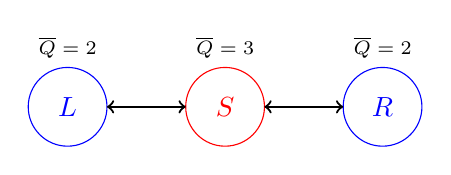
\begin{tikzpicture}
	\draw[blue] (-2,0) circle[radius=0.5] node {$L$};
	\draw[red] (0,0) circle[radius=0.5] node {$S$};
	\draw[blue] (2,0) circle[radius=0.5] node {$R$};
	
	\draw[<->,thick] (-1.5,0) -- (-0.5,0);
	\draw[<->,thick] (0.5,0) -- (1.5,0);
	
	\node at (-2,.75) {\scriptsize$\hardcapacity=2$};
	\node at (0,.75) {\scriptsize$\hardcapacity=3$};
	\node at (2,.75) {\scriptsize$\hardcapacity=2$};
\end{tikzpicture}
		\end{center}
		\caption{Macroscopic representation of station $S$ with tracks $L$ on its left and $R$ on its right.}\label{fig:example_macro}
	\end{subfigure}\vspace{2em}
	\begin{subfigure}[ht]{\textwidth}
		\begin{center}
			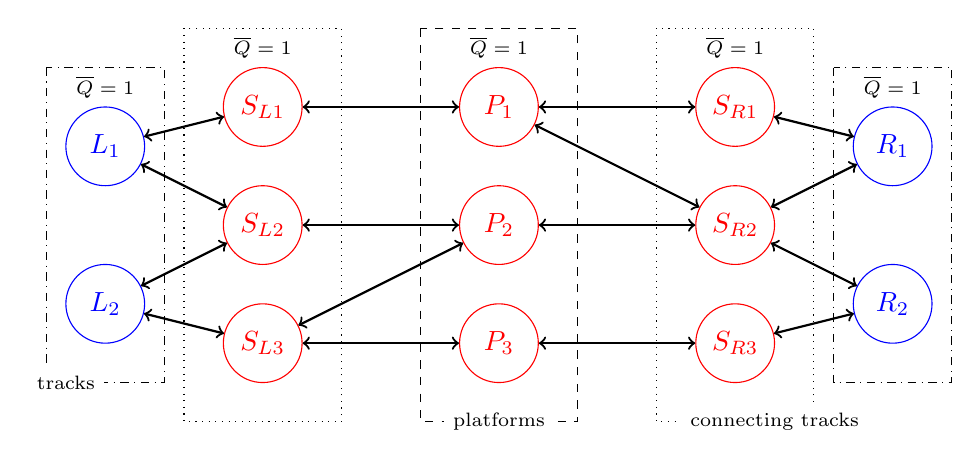
\begin{tikzpicture}
	\tikzstyle{vertex}=[circle,draw,inner sep=0pt, minimum size=1cm]
	
	\node[vertex,blue] at (-5,1) (l1) {$L_1$};
	\node[vertex,blue] at (-5,-1) (l2) {$L_2$};
	
	\node[vertex,red] at (-3,1.5) (sl1) {$S_{L1}$};
	\node[vertex,red] at (-3,0) (sl2) {$S_{L2}$};
	\node[vertex,red] at (-3,-1.5) (sl3) {$S_{L3}$};
	
	\node[vertex,red] at (0,1.5) (p1) {$P_1$};
	\node[vertex,red] at (0,0) (p2) {$P_2$};
	\node[vertex,red] at (0,-1.5) (p3) {$P_3$};
	
	\node[vertex,red] at (3,1.5) (sr1) {$S_{R1}$};
	\node[vertex,red] at (3,0) (sr2) {$S_{R2}$};
	\node[vertex,red] at (3,-1.5) (sr3) {$S_{R3}$};
	
	\node[vertex,blue] at (5,1) (r1) {$R_1$};
	\node[vertex,blue] at (5,-1) (r2) {$R_2$};
	
	\draw[<->,thick] (l1) -- (sl1);
	\draw[<->,thick] (l1) -- (sl2);
	\draw[<->,thick] (l2) -- (sl2);
	\draw[<->,thick] (l2) -- (sl3);
	
	\draw[<->,thick] (sl1) -- (p1);
	\draw[<->,thick] (sl2) -- (p2);
	\draw[<->,thick] (sl3) -- (p2);
	\draw[<->,thick] (sl3) -- (p3);
	
	\draw[<->,thick] (p1) -- (sr1);
	\draw[<->,thick] (p1) -- (sr2);
	\draw[<->,thick] (p2) -- (sr2);
	\draw[<->,thick] (p3) -- (sr3);
	
	\draw[<->,thick] (sr1) -- (r1);
	\draw[<->,thick] (sr2) -- (r1);
	\draw[<->,thick] (sr2) -- (r2);
	\draw[<->,thick] (sr3) -- (r2);
	
	\draw[dashed] (-1,2.5) rectangle (1,-2.5);
	\node[fill=white] at (0,-2.5) {\scriptsize platforms};
	
	\draw[dotted] (-4,2.5) rectangle (-2,-2.5);
	\draw[dotted] (2,2.5) rectangle (4,-2.5);
	\node[fill=white] at (3.5,-2.5) {\scriptsize connecting tracks};
	
	\draw[dashdotted] (-5.75,2) rectangle (-4.25,-2);
	\draw[dashdotted] (4.25,2) rectangle (5.75,-2);
	\node[fill=white] at (-5.5,-2) {\scriptsize tracks};
	
	\node at (-5,1.75) {\scriptsize$\hardcapacity=1$};
	\node at (-3,2.25) {\scriptsize$\hardcapacity=1$};
	\node at (0,2.25) {\scriptsize$\hardcapacity=1$};
	\node at (3,2.25) {\scriptsize$\hardcapacity=1$};
	\node at (5,1.75) {\scriptsize$\hardcapacity=1$};
\end{tikzpicture}
		\end{center}
		\caption{Microscopic representation of the same station as in \Cref{fig:example_macro}, with all platforms and physical tracks modelled explicitly.}\label{fig:example_micro}
	\end{subfigure}
	\vspace{1em}
	\caption{Differences between the micro- and macroscopic representations of a station. $\hardcapacity$ represents the capacity of a resource.}
\end{figure}

We identified certain properties that apply to all resources, no matter what parts of the physical network they represent:
\begin{itemize}
  \item Every node $\node \in \Nodes$ has an ideal (or \emph{soft}) capacity $\softcapacity_\node \in \Nat$ and a \emph{hard} capacity $\hardcapacity_\node \in \Nat$. The capacity of a resource indicates the number of trains that can occupy it at the same time. While the soft capacity can be violated (by possibly paying a certain penalty) the hard capacity cannot be violated under any circumstances. The relation $\softcapacity_\node \leq \hardcapacity_\node$ holds.
  \item Every node $\node \in \Nodes$ also has an associated boolean parameter, $\canovertake_\node \in \{0,1\}$, that indicates whether overtaking and crossing between trains can happen at the node.
\end{itemize}

The arcs in set $\Arcs$ represent the possibility for trains to move from one node to another. Arcs also have capacities, indicating the number of trains that can simultaneously transit from the source to the destination node of the arc: we indicate the capacity of $\arc \in \Arcs$ with $\hardcapacity_\arc \in \Nat$. This quantity is considered as a hard capacity.

The other main actors of a train network are, naturally, trains. Let $\Trains$ be the set of trains and consider the following properties that link together resources and trains:
\begin{itemize}
  \item Given a train $\train \in \Trains$ and a resource $\node \in \Nodes$, we give the minimum and maximum \emph{travel times}, i.e., the minimum and maximum times that $\train$ is allowed to occupy $\node$. We denote these values with $\mintraveltime_{\train,\node}$ and $\maxtraveltime_{\train,\node}$ respectively. The physical meaning of these quantities can vary depending on what the resource models. In case of a section of track, $\mintraveltime_{\train,\node}$ is given by the length of the track and the maximum speed that the train can achieve on that track. On the other hand, in case of a platform, $\mintraveltime_{\train,\node}$ is the dwelling time.
  \item Given a resource $\node \in \Nodes$, we denote with $\headway_\node$ the minimum \emph{headway} at $v$, i.e., the time that must elapse between two trains occupying the resource.
\end{itemize}

The nominal timetable describes the ideal operational status of the network. Each train $\train \in \Trains$ has a predefined path in the network,  denoted as $\trainpath_\train = (\node_1, \node_2, \ldots, \node_{k_\train})$, which is simply a sequence of resources to be visited: $\node_1, \ldots, \node_{k_\train} \in \Nodes$.

For each node in the path of train $\train$, the nominal timetable also provides the times at which the train is supposed to enter and leave the node. These times are denoted as $\intime_{\train,\node_j}$ and $\outtime_{\train,\node_j}$ respectively.

The current train plan describes the network as it is at the present moment --- and as it is forecast to be in the future, given the information available. For this reason, such a plan is also called the \emph{forecast timetable}. In an ideal scenario, the forecast timetable is always equal to the nominal one. In practice, when a disturbance or a disruption occurs, the forecast diverges from the nominal timetable.

The forecast timetable has a formal structure which is similar to that of the nominal timetable: it gives a sequence of nodes that each train must visit, together with the expected in- and out-times. Since both timetables describe the (ideal and real, respectively) situation of the network before the dispatcher takes any decision regarding rerouting, the train paths must be the same in both.

The only new parameters associated with the forecast are, therefore, the in- and out-times. To account for the uncertainty that comes with the real-time situation of the network, we actually give pairs of minimum and maximum possible in- and out-times. These values should be considered as hard values, i.e., the train cannot possibly enter a node before the minimum in-time or after the maximum in-time.

The minimum in- and out-times are denoted, respectively, as $\minintime_{\train,\node_j}$ and $\minouttime_{\train,\node_j}$, for $j = 1, \ldots, k$. The maximum in- and out-times are $\maxintime_{\train,\node_j}$ and $\maxouttime_{\train,\node_j}$.

As we mentioned in \Cref{sec:timetables}, rescheduling a train can involve rerouting it. This means that the dispatcher is allowed to change the path of the train in the network. In our model, we assume that it is only possible to choose detours from a predefined set available for each train. The set of detours associated with train $\train$ is $\Detours_\train$.

A detour is nothing more than a path in the network, so an element $\detour \in \Detours_\train$ contains a sequence of nodes: $\detour = (\node_1, \node_2, \ldots, \node_k)$. We only require that both the first and the last node of the detour are also part of the original train path $\trainpath_\train$. Furthermore, similarly to what we have seen for the current train plan, maximum and minimum in- and out-times are given for each node $\node_j$ of the detour. These are denoted as $\minintime_{\train,\detour,\node_j}$ (minimum in-time), $\maxintime_{\train,\detour,\node_j}$ (maximum in-time), $\minouttime_{\train,\detour,\node_j}$ (minimum out-time), and $\maxouttime_{\train,\detour,\node_j}$ (maximum out-time).

\subsection{Time-space graph}\label{ssec:timespace}

\begin{figure}
	\begin{center}
		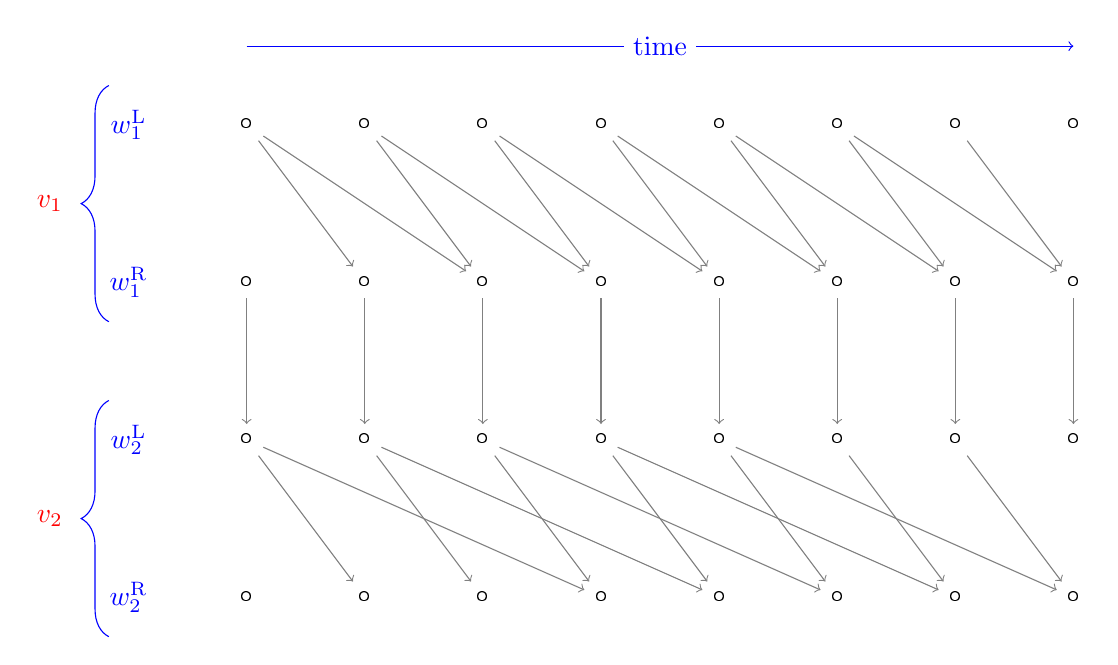
\begin{tikzpicture}
	\usetikzlibrary{decorations.pathreplacing}
	
	\node[red] at (-1,5) {$\node_1$};
	\node[red] at (-1,1) {$\node_2$};
	
	\draw[blue,decorate,decoration={brace,mirror,amplitude=10pt}] (-0.25,6.5) -- (-0.25,3.5);
	\draw[blue,decorate,decoration={brace,mirror,amplitude=10pt}] (-0.25,2.5) -- (-0.25,-0.5);
	
	\node[blue] at (0,6) {$\stnode^\textup{L}_1$};
	\node[blue] at (0,4) {$\stnode^\textup{R}_1$};
	\node[blue] at (0,2) {$\stnode^\textup{L}_2$};
	\node[blue] at (0,0) {$\stnode^\textup{R}_2$};
	
	\draw[->,blue] (1.5,7) -- (12,7) node[midway,fill=white] {time};
	
	\foreach \x in {1,...,8}
		\foreach \y in {0,...,3}
			\node at (1.5*\x,2*\y) (n\x\y) {\textopenbullet};
			
	\foreach \x in {1,...,6}
	{
		\pgfmathtruncatemacro{\r}{\x+1};
		\pgfmathtruncatemacro{\s}{\x+2};
		\draw[black!50,->] (n\x3) -- (n\r2);
		\draw[black!50,->] (n\x3) -- (n\s2);
	}
	\draw[black!50,->] (n73) -- (n82);
	
	\foreach \x in {1,...,8}
	{
		\draw[black!50,->] (n\x2) -- (n\x1);
	}
	
	\foreach \x in {1,...,5}
	{
		\pgfmathtruncatemacro{\r}{\x+1};
		\pgfmathtruncatemacro{\s}{\x+3};
		\draw[black!50,->] (n\x1) -- (n\r0);
		\draw[black!50,->] (n\x1) -- (n\s0);
	}
	\draw[black!50,->] (n61) -- (n70);
	\draw[black!50,->] (n71) -- (n80);
\end{tikzpicture}
	\end{center}
	\caption{Example of a portion of time expanded graph.}\label{fig:time_exp}
\end{figure}

The network graph $\NetGraph = (\Nodes, \Arcs)$ introduced in \Cref{ssec:network} does not explicitly model the time component. In this subsection, we present a time-space graph and we construct it starting from $\NetGraph$ and augmenting the number of nodes to take into account time and entry/exit points of nodes of $\Nodes$. Time-expanded graphs have already been used to model railway networks, e.g., in \citet{Caprara2002} and \citet{Cacchiani2010}. The \emph{time-space (di)graph} of a train $\train \in \Trains$ is denoted as $\STGraph^\train = (\STNodes^\train, \STArcs^\train)$ and is obtained in the following way.

For every entry and exit point of every node $\node \in \Nodes$, a node is added to $\STNodes^\train$. The definition of entry and exit point is strongly dependent on the physical resource modelled by $\node$. For example, if $\node$ represents a set of parallel tracks, there will be one entry and one exit point for each track; if $\node$ models a station, there would be an entry and one exit point for every track running through the station. In general, the number of entry and exit point does not need to match (e.g., a station could have more tracks one side than the other). The names \emph{entry} and \emph{exit} are only used to distinguish two physical locations on the resource, but since trains can generally run on a resource in both directions, a specific train could actually enter the resource from one of its exit points and leave it from one of the entry points.

We then need to model time into the graph. In order to do this, we first have to decide a reasonable time horizon and a time discretisation. In practical applications, these values could be provided to the model by the upstream conflict detection system. Notice, though, that the flexibility bundled with our model allows us to use different time discretisations in different parts of the time-space graph: some resources or some time intervals can be modelled with a more precise time discretisation than others. For example, it is possible to have a denser time discretisation for peak times and a sparser one for low-congestion times (e.g., at night). A denser discretisation might also be necessary for short tracks, where the travelling time could be shorter than the standard time interval. Once the time discretisation and the time horizon have been fixed, each node gets one further copy per time instant.

Finally, two dummy nodes $\source^\train$ and $\sink^\train$ are added to each graph $\STGraph^\train$. They represent, respectively, a source and sink node used as the start and end point of the train's path in the graph.

Arcs are created between pairs of nodes $(\stnode_1, \stnode_2) \in \STNodes^\train$ and they are divided in three types. The first type links nodes which represent entry and exit point relative to the same resource $\node \in \Nodes$. Such an arc would model the travelling of a train along the resource modelled by $\node$, when the difference in time instants represents a feasible travelling time for train $\train$.

The second type links nodes which represent entry and exit points of adjacent resources, that is of nodes $\node_1,\node_2 \in \Nodes$ such that $(\node_1,\node_2) \in \Arcs$. Such an arc would model a train that leaves a resource and (instantaneously) reaches a new one.

Finally, the third type links the source and the sink to the other nodes. Let $\sstnode^\train$ and $\estnode^\train$ be the entry points that train $\train$ has to use to access and leave, respectively, its start and end resources. We then add to the arc set $\STArcs^\train$ a:
 \begin{inparaenum}[(a)]
	 \item arcs from $\source^\train$ to nodes of the form $(\sstnode^\train, \timeinstant)$, where $\timeinstant$ is a time instant;
	 \item arcs from nodes of the form $(\estnode^\train, \timeinstant)$ to $\sink^\train$, where $\timeinstant$ is a time instant;
	 \item arcs from nodes of the form $(\stnode, T)$ to $\sink^\train$, where $\stnode$ is any entry or exit point, and $T$ is the last time instant of the time horizon, used to represent a train that could not reach its destination within the time horizon considered.
 \end{inparaenum}

We list the three type of arcs separately and let $\STArcs^\train = \STArcs^{\train,1} \cup \STArcs^{\train,2} \cup \STArcs^{\train,3}$, where the three sets contain, respectively, arcs of the three types listed above.

\Cref{fig:time_exp} shows a portion of a time-expanded graph. Nodes $\stnode^\textup{L}_1$ and $\stnode^\textup{R}_1$ are the left and right extreme points of $\node_1 \in \Nodes$, while nodes $\stnode^\textup{L}_2$ and $\stnode^\textup{R}_2$ are the left and right extreme points of $\node_2 \in \Nodes$. The arcs between $\stnode^\textup{L}_1$ and $\stnode^\textup{R}_1$ represent the traversal of resource $\node_1$ and, analogously, the arcs between $\stnode^\textup{L}_2$ and $\stnode^\textup{R}_2$ represent the traversal of resource $\node_2$. Different arcs having the same source node model the different travelling times associated to different speeds. The vertical arcs between $\stnode^\textup{R}_1$ and $\stnode^\textup{L}_2$ represent the possibility of moving from $\node_1$ to $\node_2$.

The arcs in $\STArcs^{\train,1}$ can be mapped back to the resources and the time intervals they represent in the following way. For each arc $\arc \in \STArcs^{\train,1}$, let $\uresource(\arc) \in \Nodes$ be the underlying resource modelled by the arc; analogously, let $\duresource(\arc) \in \Nodes \times \{ -1, +1 \}$ be the directed underlying resource, used to distinguish the direction in which the resource is being traversed; let $\reslength(\arc)$ be the length of the associated resource $\uresource(\arc)$. Let also $\stime(\arc)$ and $\etime(\arc)$ be the start and end time of arc $\arc$, i.e. the times when the train (respectively) occupies and frees the resource.

\subsection{Constraints}\label{ssec:conflicts}

As defined in \Cref{sec:introduction}, conflicts are those situations that either can't physically happen or that would compromise the safety of operations, and their resolution plays the same role as satisfying a constraint in a Mixed Integer Programme (MIP). In order to give a more precise description of the contraints presented in the rest of this section, we give some mathematical formulation in which we use the notation $x^\train_\arc \in \{0,1\}$ as a variable in a Mixed Integer Programme, having value 1 iff the arc $\arc \in \STArcs^\train$ is part of the path of train $\train$.

Preliminary experiments with solving a compact MIP formulation of real-life instances with a commercial solver have shown that model generation alone can take several minutes, and solving the root node requires more than a day. For this reason, we do not include a complete MIP model for the problem we are presenting. Rather, the notation $x^\train_\arc$ should be seen as a way to describe precisely the constraints taken into account by our algorithm, and how they are reflected on the time-space graph.

Notice, first of all, that a train schedule can be modelled as a path in $\STGraph^\train$, starting in $\source^\train$ and ending in $\sink^\train$ and abiding to the usual flow conservation constraint. Formally, this means that:
\begin{align}
  \sum_{\arc \in \STArcs^{\train,+}(\source^\train)} x_\arc^\train = 1 \\
  \sum_{\arc \in \STArcs^{\train,-}(\sink^\train)} x_\arc^\train = 1 \\
	\sum_{\arc \in \STArcs^{\train,-}(\stnode)} x_\arc^\train =%
  \sum_{\arc \in \STArcs^{\train,+}(\stnode)} x_\arc^\train & \quad &%
	\forall \stnode \in \STNodes^\train \setminus \{ \source^\train, \sink^\train \}
\end{align}
where $\STArcs^{\train,+}(\stnode)$ (resp. $\STArcs^{\train,-}(\stnode)$) is the set of all arcs outgoing from (resp. incoming to) node $\stnode \in \STNodes^\train$.

In this work we deal with the rescheduling of the trains once the conflicts have already been detected and reported, so we will assume that the complete list of conflicts is available together with the current train plan. In other words, the conflict detection system works upstream of our system. This assumption is not restrictive, as a simple linear-time algorithm over the current train plan is able to produce the complete list of conflicts.

The presence of conflicts could be formally detected by checking for violations in (hard) constraints involving the variables $x^\train_\arc$. As we will see in \Cref{ssec:objective_function}, we want to penalise the violation of certain soft constraints. In a MIP model, for example, a hard capacity limit can be enforced via a constraint, whereas the extent of the violation of a soft capacity limit can be penalised, by introducing an auxiliary variable that plays the role of the slack variable relative to the constraint.

\subsubsection{Illegal crossing and overtake}

\begin{figure}
	\begin{center}
		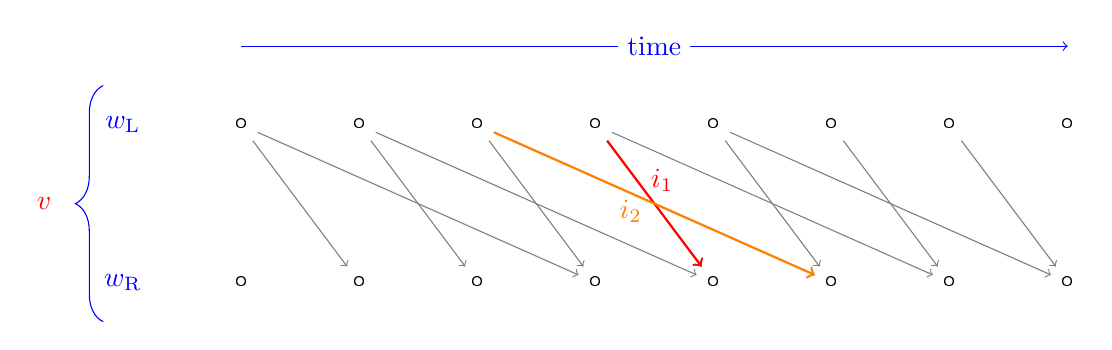
\begin{tikzpicture}
	\usetikzlibrary{decorations.pathreplacing}
	
	\node[red] at (-1,1) {$\node$};
	
	\draw[blue,decorate,decoration={brace,mirror,amplitude=10pt}] (-0.25,2.5) -- (-0.25,-0.5);
	
	\node[blue] at (0,2) {$\stnode_\textup{L}$};
	\node[blue] at (0,0) {$\stnode_\textup{R}$};
	
	\draw[->,blue] (1.5,3) -- (12,3) node[midway,fill=white] {time};
	
	\foreach \x in {1,...,8}
		\foreach \y in {0,...,1}
			\node at (1.5*\x,2*\y) (n\x\y) {\textopenbullet};
			
	\foreach \x in {1,...,5}
	{
		\pgfmathtruncatemacro{\r}{\x+1};
		\pgfmathtruncatemacro{\s}{\x+3};
		\draw[black!50,->] (n\x1) -- (n\r0);
		\draw[black!50,->] (n\x1) -- (n\s0);
	}
	\draw[black!50,->] (n61) -- (n70);
	\draw[black!50,->] (n71) -- (n80);
	
	\draw[red,thick,->] (n41) -- (n50) node[midway,xshift=0.1cm,yshift=0.3cm] {$\train_1$};
	\draw[orange,thick,->] (n31) -- (n60) node[midway,xshift=-0.3cm,yshift=-0.1cm] {$\train_2$};
\end{tikzpicture}
	\end{center}
	\caption{Train $i_1$ overtaking train $i_2$ on resource $v$. Notice how this situation corresponds to crossing arcs in the time-space graph.}\label{fig:overtake}
\end{figure}

An illegal crossing (overtake) describes a situation when a train would cross (overtake) with another one, on a resource $\node$ where this is illegal, i.e. $\canovertake_\node = 0$. An example of overtaking is described in \Cref{fig:overtake}.

An overtake corresponds to the violation of the following constraints: for each train $\train$, each resource $\node$ where overtaking is forbidden, and each arc $\arc \in \STArcs^{\train,1}$ such that $\uresource(\arc) = \node$:
\begin{equation}
  \sum_{\substack{\trainn \in \Trains \\ \trainn \neq \train}}%
  \sum_{\substack{%
    \arc' \in \STArcs^{\trainn,1} \\%
    \duresource(\arc') = \duresource(\arc), \\%
    \stime(\arc') > \stime(\arc), \\%
    \etime(\arc') \leq \etime(\arc)%
  }}%
  x_{\arc'}^\trainn + x_\arc^\train \leq 1 \label{eq:overtake}
\end{equation}
\Cref{eq:overtake} states that train $\trainn$ overtakes train $\train$ on resource $\node$ if $\trainn$ arrives in $\node$ after $\train$, but leaves $\node$ before $\train$, and both trains travel in the same direction.

Analogously, corresponds to the violation of the following contraints: for each train $\train$, each resource $\node$ on which crossing is forbidden, and each arc $\arc \in \STArcs^{\train,1}$ such that $\uresource(\arc) = \node$:
\begin{equation}
  \sum_{\substack{\trainn \in \Trains \\ \trainn \neq \train}}%
  \sum_{\substack{%
    \arc' \in \STArcs^{\trainn,1} \\%
    \uresource(\arc') = \uresource(\arc), \\%
    \duresource(\arc') \neq \duresource(\arc), \\%
    \etime(\arc) \geq \stime(\arc')%
  }}%
  x_{\arc'}^\trainn + x_\arc^\train \leq 1 \label{eq:crossing}
\end{equation}
\Cref{eq:crossing} states that train $\trainn$ crosses train $\train$ on resource $\node$ if $\trainn$ arrives in $\node$ before $\train$ has left, and the two trains travel in opposite directions.

\subsubsection{Capacity violation}

A capacity violation occurs when the number of trains simultaneously occupying a resource is greater of the hard capacity of the resource. Such a conflict corresponds to a violated inequality of the following type:
\begin{equation}
  \sum_{\train \in \Trains}%
  \sum_{\substack{%
    \arc \in \STArcs^\train \\%
    \uresource(\arc) = \node, \\%
    \stime(\arc) \leq \timeinstant, \\%
    \etime(\arc) \geq \timeinstant%
  }}%
  x_\arc^\train \leq \hardcapacity_\node
\end{equation}
for each resource $\node$ and each time instant $\timeinstant$, where we remind that $\hardcapacity_\node$ is the hard capacity of resource $\node$.

\subsubsection{Headway violation}

Such a conflict occurs when a train occupies a resource that has been occupied by another train, and not enough time has elapsed between the first train leaving the resource and the second one entering it. For each train $\train \in \Trains$ and each arc $\arc \in \STArcs^{\train,1}$ corresponding to a resource $\uresource(\arc)$ on which crossing and overtaking is forbidden ($\canovertake_{\uresource(\arc)} = 0$, as otherwise the headway must not be respected), a headway conflict corresponds to a violated constraint:
\begin{equation}
	\sum_{\substack{%
		\trainn \in \Trains \\%
		\trainn \neq \train%
	}}%
	\sum_{\substack{%
		\arc' \in \STArcs^{\trainn,1} \\%
		\uresource(\arc') = \uresource(\arc) \\%
		\etime(\arc') \geq \stime(\arc) - \headway_{\resource(\arc)} \\%
		\stime(\arc') \leq \etime(\arc) + \headway_{\resource(\arc)}%
	}}%
	x_{\arc'}^\trainn + x_\arc^\train \leq 1
\end{equation}

\subsubsection{Time dependencies}\label{ssec:time_dependencies}

Avoiding the conflicts described in the previous subsection is usually enough to come up with a new plan that allows safe operations and limits the deviations from the nominal timetable. Unfortunately, this is not always enough to provide a holistic, good solution.

Consider, for example, a passenger on a delayed train that risks missing his connection. From his point of view, a solution that also delays his next train (to ``wait for him'') is preferable to a solution that does not. But from a train operator's point of view, a solution that does not delay the second train may be considered better, since no delay is better than some delay.

Then, if the train operator's \emph{service intention} is, for example, ``moving passengers from A to B'' (even at the cost of increasing the overall delay, to some extent), this should be taken into account by the rescheduling algorithm.

In order to take into account service intentions, we introduce the concept of \emph{time dependencies} (\citet{Caimi2011}).
A time dependency is a relationship of precedence between two events happening in the network. For example, a time dependency could mandate that the event ``train $\train_1$ leaves node $\node$'' can only happen a certain time after the event ``train $\train_2$ arrives at node $\node$''; intuitively, we would say that train $\train_1$ needs to wait for train $\train_2$ at node $\node$.

\begin{figure}
	\begin{center}
		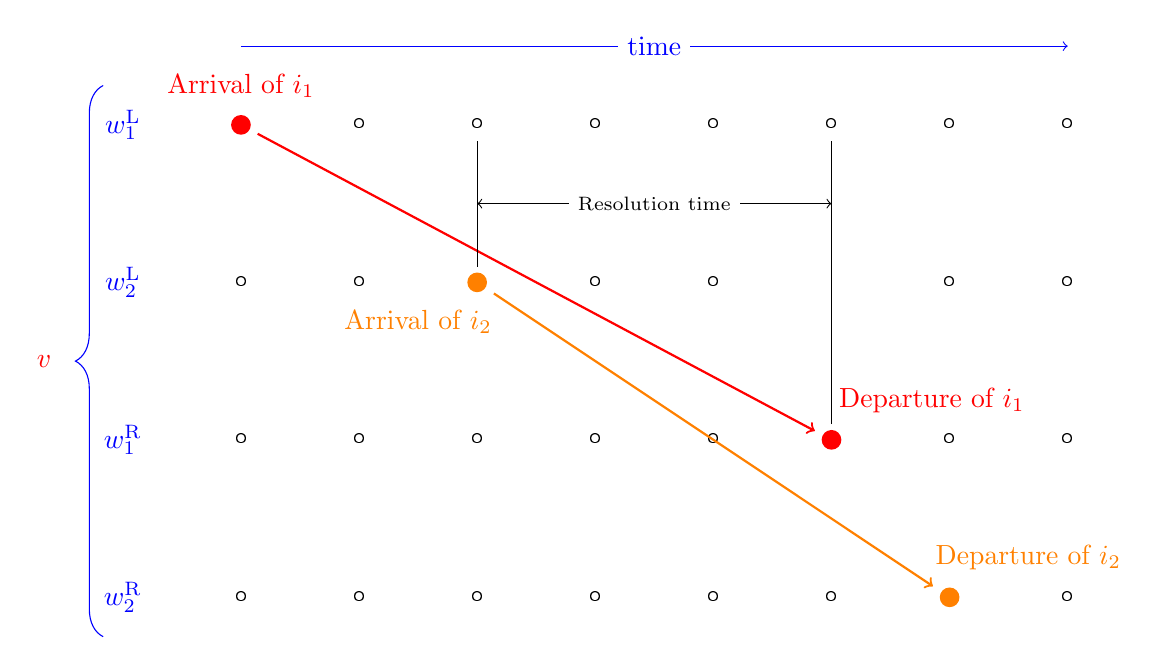
\begin{tikzpicture}
	\usetikzlibrary{decorations.pathreplacing}
	\usetikzlibrary{positioning}
	
	\node[red] at (-1,3) {$\node$};
	
	\draw[blue,decorate,decoration={brace,mirror,amplitude=10pt}] (-0.25,6.5) -- (-0.25,-0.5);
	
	\node[blue] at (0,6) {$\stnode^\textup{L}_1$};
	\node[blue] at (0,4) {$\stnode^\textup{L}_2$};
	\node[blue] at (0,2) {$\stnode^\textup{R}_1$};
	\node[blue] at (0,0) {$\stnode^\textup{R}_2$};
	
	\draw[->,blue] (1.5,7) -- (12,7) node[midway,fill=white] {time};
	
	\foreach \x in {1,...,8} {
		\foreach \y in {0,...,3} {
			\ifthenelse{6 = \x \AND 2 = \y}{}{\node at (1.5*\x,2*\y) (n\x\y) {\textopenbullet};}
		}
	}
	
	\tikzstyle{relevant}=[circle,fill,minimum size=0.25cm,inner sep=0pt];
	\node[relevant,red] at (1.5,6) (arr1) {};
	\node[relevant,red] at (9,2) (dep1) {};
	\node[relevant,orange] at (4.5,4) (arr2) {};
	\node[relevant,orange] at (10.5,0) (dep2) {};

	\node[red,above=0.025cm of n13] {Arrival of $\train_1$};
	\node[red,above=0.02cm of n61,xshift=1.275cm] {Departure of $\train_1$};
	\node[orange,below=0.025cm of n32,xshift=-0.75cm] {Arrival of $\train_2$};
	\node[orange,above=0.025cm of n70,xshift=1cm] {Departure of $\train_2$};

	\draw[red,thick,->] (n13) -- (n61);
	\draw[orange,thick,->] (n32) -- (n70);
	
	\draw (n32) -- (n33);
	\draw (n61) -- (n63);
	
	\draw[<->] (4.5,5) -- (9,5) node[midway,fill=white] {\scriptsize Resolution time};
\end{tikzpicture}
	\end{center}
	\caption{Resolution time of a time dependency between the arrival of train $\train_2$ and the departure of train $\train_1$ at a station.}\label{fig:dependency}
\end{figure}

A service intention can merely suggest a precedence between events, as in the case of passenger connections: it is preferable that the connection is kept, but this ``promise'' can be broken in order to improve the overall quality of service. On the other hand, the precedence can also be mandatory, as in the case of two trains that share crew or rolling stock.

Let $\Dependencies$ be the set of time dependencies. We associate to each element $\dependency \in \Dependencies$ the following values:
\begin{itemize}
  \item The two trains $\train_{\dependency,1},\train_{\dependency,2}$ involved in the dependency.
  \item The two resources $\node_{\dependency,1},\node_{\dependency,2}$ at which the linked events need to take place, respectively.
  \item Two parameters $\dependencytype_{\dependency,1},\dependencytype_{\dependency,2} \in \{0,1\}$ that take value $0$ if the corresponding event is an arrival or value $1$ if it is a departure.
  \item A parameter $\mandatory_\dependency \in \{0,1\}$ that takes value $1$ iff the dependency is mandatory.
  \item The minimum and maximum resolution time, $\minrestime_\dependency$ and $\maxrestime_\dependency$. The dependency is considered satisfied if the two events take place at least $\minrestime_\dependency$ and at most $\maxrestime_\dependency$ time units apart.
  \item For non-mandatory (also called \emph{logical}) time dependencies, we give a maximum waiting time $\waittime_\dependency$. The dependency must be satisfied if it is possible to do so by introducing at most $\waittime_\dependency$ time units of delay. If this cannot be done, the dependency can either be satisfied or not. For example, in the case of a connection between two trains, we might require that a train waits for the other at most $\waittime_\dependency$ time units. If the required wait is greater, the train can decide to break the connection.
\end{itemize}

\Cref{fig:dependency} shows an example in which train $\train_1$ stays at station $\node$ for three time intervals after the arrival of train $\train_2$, presumably to \emph{wait} for passengers travelling on $\train_2$. The resources $\stnode_k^\textup{L},\stnode_k^\textup{R}$ represent entry and exit points of two platform at the station ($k = 1,2$).

The violation of a mandatory time dependency $\dependency \in \Dependencies$ can be detected as follows. Assume wlog that the event relative to train $\train_{\dependency,1}$ needs to take place before the event relative to train $\train_{\dependency,2}$. For $k = 1,2$ and $\arc \in \STArcs^{\train_{\dependency,k},1}$ such that $\uresource(\arc) = \node_{\dependency,k}$, consider the parameter:
\begin{equation*}
  \deptime_{\dependency,k}(\arc) =  \begin{cases}
                                      \stime(\arc) & \text{ if } \dependencytype_{\dependency,k} = 1 \\
                                      \etime(\arc) & \text{ if } \dependencytype_{\dependency,k} = 0
                                    \end{cases}
\end{equation*}
  We can then formulate the corresponding constraint:
\begin{equation}
  \minrestime_\dependency \leq%
  \sum_{\substack{%
    \arc \in \STArcs^{\train_{\dependency,2},1} \\%
    \uresource(\arc) = \node_{\dependency,2}%
  }}%
  x_\arc^\train \deptime_{\dependency,2}(\arc) -
  \sum_{\substack{%
    \arc \in \STArcs^{\train_{\dependency,1},1} \\%
    \uresource(\arc) = \node_{\dependency,1}%
  }}%
  x_\arc^\train \deptime_{\dependency,1}(\arc)%
  \leq \maxrestime_\dependency
\end{equation}

\subsubsection{Split and merge}

Similar to time dependencies are split and merge operations. These are events in which the trains that enter a node are not the same that leave it. They model real-life operations such as decoupling some cars from a train, so that they can get a new locomotive and proceed to a different destination.

In the most general version, any number of trains can enter a certain node and any number of trains can leave it, so a split/merge is identified by a node $\node \in \Nodes$ and two sets of trains $\Trains_1,\Trains_2 \subset \Trains$ that represent in-trains and out-trains. The out-trains can leave the node only after a certain amount of time has passed since the last in-train reached it. This time accounts, in practice, for the time necessary to perform any physical coupling and decoupling, or to change crew or rolling stock. Special cases of split/merge operations are:
\begin{itemize}
	\item \emph{Split}, when one train enters the node, and two or more exit it.
	\item \emph{Merge}, when more than one train enter the node, and only one exits it.
	\item \emph{Rename}, when one train enters the node and one train exits it.
\end{itemize}
In case of split/merge events, the node's capacity is not considered, as it is assumed that it is always feasible for the event to take place in the node specified. Finally, note that these events are mandatory: for example, it is not possible that a train will be detoured around a node in which it has to undergo a split.

In the following we show how a split or merge operation can be modelled in terms of mandatory time dependencies; in this way, the conflict resulting from a missed split or merge can be detected by checking for the violation of the corresponding time dependency constraint. For example, if train $\train$ needs to be split into trains $\train', \train''$ at resource $\node$, then said resource will be set as the destination of $\train$ and the origin of $\train'$ and $\train''$. Furthermore, two dependencies will be created:
\begin{itemize}
	\item $\dependency' \in \Dependencies$ links trains $\train$ and $\train'$ and has: $\train_{\dependency',1} = \train, \train_{\dependency',2} = \train'$; $\node_{\dependency',1} = \node_{\dependency',2} = \node$; $\dependencytype_{\dependency',1} = 0, \dependencytype_{\dependency',2} = 1$; $\mandatory_{\dependency'} = 1$; $\minrestime_{\dependency'}$ will be the time needed to perform the split operation; $\maxrestime_{\dependency'}$ will be the maximum time allowed for the split to take place, if any.
	\item $\dependency'' \in \Dependencies$, analogously links trains $\train$ and $\train''$.
\end{itemize}

\subsubsection{Maximum and minimum entry, exit, and travel times}

Maximum and minimum entry, exit, and travel times can be enforced by removing from the graphs $\STGraph^\train$ those nodes that would correspond to an infeasible (resource, time) couple. For example, if a train $\train \in \Trains$ cannot enter resource $\node$ before time $\timeinstant$, all nodes of $\STNodes^\train$ corresponding to resource $\node$ at a time $t' < t$ can be removed from the graph. Analogously, if the minimum travel time along a resource $\node$ is $\timeinstant$, all arcs $\arc \in \STArcs^{\train,1}$ such that $\etime(\arc) - \stime(\arc) < \timeinstant$ can be removed.

\subsection{Objective function}\label{ssec:objective_function}

The objective value can be written as a function of the paths in the time-space graphs, and therefore of $\vec{x} = (x_\arc^\train)$, in the following way:
\begin{equation}
  f(\vec{x}) = f_1(\vec{x}) + f_2(\vec{x}) + f_3(\vec{x}) + f_4(\vec{x}) \label{eq:objf}
\end{equation}
The four components correspond to delays, logical dependency breaking, soft capacity violations, and the use of detours. Each of these components represents a sum of penalties that quantify how undesirable it is to incur in the corresponding violations. The penalty, therefore, is not only limited to represent the economical disadvantage of taking a particular decision (e.g., increased energy consumption) but can also represent intangible values, such as customer satisfaction. In the following, we analyse these four components.

\subsubsection{Delays}

In the nominal timetable, we associated to each train $\train$ and each resource $\node_j$ in the train's path, an ideal in-time $\intime_{\train, \node_j}$ and an ideal out-time $\outtime_{\train, \node_j}$. Any deviation from these times can be penalised, by considering two piecewise-linear functions that respectively assign a cost to delays in arriving at and departing from the resource. These penalty functions are denoted as $\indelaypenalty_{\train,\node_j}(\cdot)$ and $\outdelaypenalty_{\train, \node_j}(\cdot)$.

Notice that this general definition allows us to assign different penalty profiles to different resources: for example, if some resource is considered critical for a train, we can assign a higher penalty to delays at that resource. The function can also operate on negative delays, allowing us to penalise trains that arrive at a node with excessive advance. Finally, further flexibility is bundled in the piecewise-linear nature of the function: for example, we might want to have a penalty that grows linearly with the delay up to a certain point, after which a big flat penalty is assigned, as any further delay does not worsen the situation any more. This could be achieved with a penalty profile such as that in \Cref{fig:example_penalty}.

\begin{figure}
  \begin{center}
    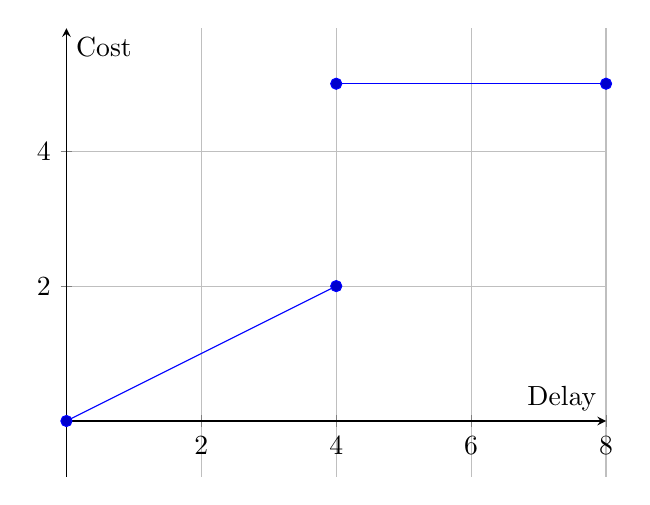
\begin{tikzpicture}
  \begin{axis}[axis lines = middle, axis equal, grid = both, xlabel = {Delay}, ylabel = {Cost}]
    \addplot coordinates{(0,0) (4,2)};
    \pgfplotsset{cycle list shift=-1} % Re-use the same style as the first plot
    \addplot coordinates{(4,5) (8,5)};
  \end{axis}
\end{tikzpicture}
  \end{center}
  \caption{Example of a penalty profile for the arrival of a train at a certain resource, with a ``jump'' in cost if the delay is greater than 4 time units.}
  \label{fig:example_penalty}
\end{figure}

\subsubsection{Dependency breaking}

As we mentioned in \Cref{ssec:time_dependencies}, logical dependencies are not mandatory and therefore we can decide to break them. In our implementation, when such a dependency $\dependency \in \Dependencies$ is broken, we pay a penalty $\dependencypenalty_\dependency$. (Notice that, in principle, a piecewise linear function could be used, as done for delays.)

\subsubsection{Capacity violations}

When we violate the soft capacity $\softcapacity_\node$ of a resource $\node$, we pay a penalty $\capacitypenalty_\node$. In our implementation, this penalty remains the same no matter how big the capacity violation is. (Notice that, in principle, a piecewise linear function could be used in this case too.)

\subsubsection{Detours}

Finally, a fixed penalty $\detourpenalty_{\detour}$ is paid when a train $i$ is re-routed along a detour $\detour \in \Detours_\train$. This penalty takes into account all the costs (economical or otherwise) incurred because of the rerouting. Dependency breaking and capacity violations are calculated separately when a detour is taken. If some node of the detour can be naturally mapped to nodes of the original path, the delay penalty can also be calculated. For example, if the detour consists of a platform change at a station, we can naturally assign to the new platform the in- and out-times at the old platform.

The penalty $\detourpenalty_{\detour}$ should be considered as a fixed cost incurred by the mere fact of having rerouted the train. It can include both \emph{real} and \emph{virtual} costs. For example, if the detour consist of a path longer than the original one, there would be increased energy costs. But if the detour also excludes a station, there would be a much increased passenger dissatisfaction. Therefore, the magnitude of the penalty depends on the type of detour: a platform change will have a small associated penalty, while a major change in the train's path will be associated with a bigger penalty.

\subsubsection{Other terms}\label{sssec:other_terms}

Even though in the present work we only consider the four components discussed above, further terms can be easily introduced in the objective function to take into account other indicators. For example:
\begin{itemize}
	\item Number of modifications with respect to the nominal timetable, eventually weighted differently depending on the nodes or trains involved. This could be done to make sure that the new timetable does not disrupt too much the current operations (i.e., changes too many train paths) just to save a few seconds of overall delay.
	\item Increased travel time on resources, eventually involving a piecewise-linear penalty profile. This term would help avoiding unnecessary stops or excessive brake-accelerate cycles, for increased passenger comfort and reduced energy consumption.
\end{itemize}

  \section{Solution Algorithm}\label{sec:solution_algorithm}

A solution to the TRP is a collection of paths, one for each train, in the time-space graph $\STGraph$. The solution algorithm must be able to modify the forecast timetable in order to solve the conflicts, and to compute the new objective function. Key requirements for this algorithm, deriving from its real-time nature, are:
\begin{itemize}
	\item It must produce solutions of high quality in very short computational times (a few seconds). This is due to the fact that the algorithm is used on-line by dispatcher, who needs reasonable advice in few seconds, to guarantee the safety of operations in the network. For this reason, we focussed on a heuristic approach.
	\item If the algorithm is not able to find a conflict-free schedule, it has to give the dispatcher a schedule with the smallest possible number of remaining conflicts. This means that solving more conflicts needs to always have priority over other factors. In order to accomplish this, we established an implicit hierarchy through our objective function. A very high penalty is assigned to each unresolved conflict, so that a solution with fewer conflicts will always prevail on one which has more, while the ``standard'' objective function is used to decide the best one between two solutions with the same number of remaining conflicts. Therefore, the objective function presented in \eqref{eq:objf} is used as a part of the overall objective function: $\tilde{f}(\vec{x}) = P \cdot N_\textup{RC}(\vec{x}) + f(\vec{x})$, where $P$ is the large penalty to pay for each conflict, and $N_\textup{RC}$ gives the number of remaining conflicts in the solution.
	\item The algorithm should allow for a high degree of parallelisation, allowing to concurrently produce multiple rescheduled timetables that will be stored in a solution pool, from which the best one will be selected. This allows the algorithm to employ and evaluate different strategies in situations where none of them is clearly superior to the others, thereby focussing on different key aspects of the problem.
\end{itemize}

With these requirements in mind, we now give a general description of the algorithm which boradly falls into the category of iterated greedy algorithms (see, e.g., \citet{Ruiz20072033}). After an initialisation phase in which trains are ranked according to some criterion, the algorithm iterates among two main phases, until a termination condition is met. The two phases are:
\begin{enumerate}
	\item \textbf{Construction}: a new timetable is obtained by rescheduling the trains one by one, according to their ranking. \label{it:con}
	\item \textbf{Shaking}: the train ranking is perturbed following a set of rules. \label{it:sha}
\end{enumerate}
In our case the termination criterion is a hard time limit, with early termination if the solutions didn't improve over a certain number of iterations. The next subsections will describe each phase in detail. Furthermore, in order to speed up the computational time of the construction phase, we employed a sparsification of the graph $\STGraph$. This is a technique used to remove some edges and vertices from the time-space graph. Its use is justified by the fact that, by choosing a fine time discretisation, we might create a great number of edges, many of which can be removed without strongly impacting the quality of the train plans.

Notice that, for the algorithm initialisation, for the shaking phase, and for sparsification we propose several possible alternatives. Therefore, an instance of our algorithm is completely defined once we specify which initial sorting, shaking policy, and sparsification method is used. An extensive experimental testing of the proposed alternatives, described in \Cref{ssec:ptuning}, will help determining well-performing combinations of the algorithm's components.

\subsection{Initial sorting}

Since the algorithm constructs a schedule for one train at a time (Step \ref{it:con}), the order in which the trains are considered is clearly important, as trains scheduled later will be constrained by those scheduled earlier. Since there is no ``natural'' order of trains, we used various sorting criteria:
\begin{itemize}
	\item \textbf{Random}: the trains are randomly sorted.
	\item \textbf{Congestion}: the trains are sorted according to the number of conflicts in their forecast timetable, putting trains with more conflicts first. The rationale behind this choice is that a train that generates a lot of conflicts is harder to schedule, and therefore should be scheduled earler. Using the notation introduced earlier, if $\vec{x}^*$ is the assignment of variables corresponding with the forecast timetable, then we sort the trains by decreasing value of $N^\train_\textup{RC}(\vec{x}^*)$, where $N^\train_\textup{RC}(\vec{x}^*)$ is the number of conflicts in train $\train$'s schedule, and $N_\textup{RC}(\vec{x}^*) = \sum_{\train \in \Trains} N^\train_\textup{RC}(\vec{x}^*)$.
	\item \textbf{Length}: the trains are sorted according to the number of nodes in their original path in decreasing order. The longer the path, in fact, the higher the chances that a conflict will be present at some node. The trains are therefore sorted in decreasing order of the size of their set $\{ \arc \in \Arcs^\train \ : \ \vec{x}^* = 1 \}$.
	\item \textbf{Conflict time}: the trains are sorted according to the time instant of the earliest conflict in their forecast timetable. This is because an early conflict can impact the overall network status at a much later time. In other words, there is more freedom when fixing conflicts happening earlier, and we want to fully use this freedom.
	\item \textbf{Speed}: the trains with highest average speed are scheduled earlier. This strategy is based on the observation that faster trains have schedules that are more sensitive to variations. The average speed of a train $\train$ is given by:
  \begin{equation*}
    \frac{
      \sum_{\arc \in \STArcs^\train, \, \vec{x}^*_\arc = 1} \frac{\reslength(\arc)}{\etime(\arc) - \stime(\arc)}%
    }{%
      \left| \left\{ \arc \in \STArcs^\train \ : \ \etime(\arc) > \stime(\arc) \text{ and } \vec{x}^*_\arc = 1 \right\} \right|%
    }
  \end{equation*}
\end{itemize}
During a preliminary experimental phase, we noticed that using the sorting criteria in reverse order can sometimes lead to better results. For this reason we also considered the criteria \textbf{Reverse congestion} and \textbf{Reverse speed}.

\subsection{Construction}\label{ssec:construction}

Each train schedule is constructed by solving a shortest-path problem on the time-expanded graph $\STGraph$, where the starting node correspons to the current position of the train and the ending node corresponds to the train's desired position at the end of the time horizon.

Since trains run along fixed routes, with only a few possible detours, and since they have hard constraints on the time at which they can reach and leave certain resources, the graph $\STGraph$ can be pruned accordingly for each train. Once this is done, the shortest path is constructed with a custom label-setting algorithm. Given a partial path to a certain node $(\stnode, \timeinstant) \in \STNodes$, the corresponding label will be $L = ((\stnode', \timeinstant'), c)$ where the node $(\stnode', \timeinstant') \in \STNodes$ is the predecessor of $(\stnode, \timeinstant)$ in the partial path and $c \in \Rea$ is the cost of the partial path up to the current node.

Notice that, since trains are scheduled sequentially and the algorith is ran on a different time-space graph for each train, we cannot run into deadlocks. A deadlock will indeed correspond to an unresolved conflict (usually a capacity violation) and be accordingly heavily penalised in the objective function.

\begin{figure}
	\begin{center}
		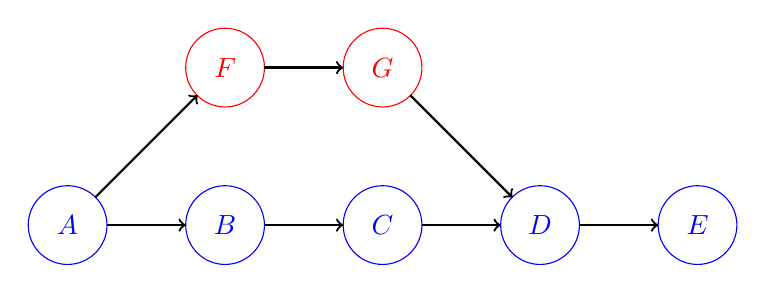
\begin{tikzpicture}
	\draw[blue] (0,0) circle[radius=0.5] node {$A$};
	\draw[blue] (2,0) circle[radius=0.5] node {$B$};
	\draw[blue] (4,0) circle[radius=0.5] node {$C$};
	\draw[blue] (6,0) circle[radius=0.5] node {$D$};
	\draw[blue] (8,0) circle[radius=0.5] node {$E$};
	\draw[red] (2,2) circle[radius=0.5] node {$F$};
	\draw[red] (4,2) circle[radius=0.5] node {$G$};
	
	\draw[->,thick] (0.5,0) -- (1.5,0);
	\draw[->,thick] (2.5,0) -- (3.5,0);
	\draw[->,thick] (4.5,0) -- (5.5,0);
	\draw[->,thick] (6.5,0) -- (7.5,0);
	\draw[->,thick] (0.35,0.35) -- (1.65,1.65);
	\draw[->,thick] (2.5,2) -- (3.5,2);
	\draw[->,thick] (4.35,1.65) -- (5.65,0.35);
\end{tikzpicture}
	\end{center}
	\caption{Topological order between nodes (resources) of a simple network.}\label{fig:toporder}
\end{figure}

We discuss now two main aspects of this algorithm: the order in which we extend the labels and how we update the cost component. Labels are extended greedily, i.e., starting from the one with the lowest cost component, but with one exception: a label related to a resource $\stnode$ will be extended only after all the labels related to resources $\stnode' \prec \stnode$ have already been extended (independently from the time interval), even if they have a higher cost. The relation $\prec$ is the topological order relation between nodes in the subgraph of $\NetGraph$ induced by the union of the path of the train $\trainpath_\train$ and all the detours in $\Detours_\train$. To better understand this rule, consider \Cref{fig:toporder}, which describes the topological setup of a network with a main corridor and a possible detour (via $F$ and $G$). Labels related to resource $D$, for example, will be extended only after all labels related to resources $A$, $B$, $C$, $F$ and $G$ have been extended, since $A \prec B \prec C \prec D$ and $A \prec F \prec G \prec D$.

The cost component is updated taking into account the various penalties included in the objective function. Some of these penalties, however, depend on the interaction between different trains. As an example, consider a connection between trains $\train_1$ and $\train_2$. If $\train_1$ is scheduled before $\train_2$, when we schedule $\train_1$ will just assume that the connection will be satisfied. If, when scheduling $\train_2$, we realise that the connection is broken, we will add the penalty on the objective function of $\train_2$.

Finally, we need to take special care in case of split/merge operations, as these require the presence of multiple trains on the same resource at the same time. When the partial path of an input train reaches one of these resources, we fix the schedule of the train up to that point, by choosing the lowest cost partial path (we first explore all non-dominated partial paths up to the synchronisation point). We proceed with the construction of the schedule for the output trains, only once all the schedules of the input trains have been fixed up to the considered resource.

\subsection{Shaking}

In the shaking phase we perturb the ordering of the trains (the \emph{dispatching sequence}) with the aim of finding an ordering which leads, through a new construction phase, to an improving solution. We present two alternative policies, inspired to two well-known metaheuristic algorithms: Reduced Variable Neighbourhood Search (RVNS) and Tabu Search (TS). As mentioned in the beginning of this section, these two alternative policies are experimentally evaluated in \Cref{sec:computational_results}.

The RVNS (see, for example, \citet{Hansen2010}) explores the solution space of the problem by employing a sequence of neighbourhood structures $\nbstruct_1, \ldots, \nbstruct_{K}$. A neighbourhood structure defines a way to describe the neighbourhood of any solution $x$ in the solution space.

Starting from a solution $x$, RVNS generates a new random solution $x' \in \nbstruct_1(x)$. If the new solution is not better than the previous one, it goes on to the second neighbourhood structure and generates a random $x' \in \nbstruct_2(x)$. The procedure continues until either we run out of neighbourhood structures or the new solution $x'$ is better than the current one $x$. In the first case, the algorithm terminates; in the second case, the algorithm is restarted using $x'$ as initial solution and going back to using $\nbstruct_1$.

The neighbourhood structures are typically such that
\begin{equation}
	\nbstruct_1(x) \subseteq \nbstruct_2(x) \subseteq \ldots \subseteq \nbstruct_K(x) \label{eq:nbstruct}
\end{equation}
for all solutions $x$. This means that while no improving solution is found, the search space around $x$ is enlarged.

In our case, the neighbourhood structure $\nbstruct_k(x)$ consist in considering all dispatching orders that can be obtained from $x$ by performing at most $k$ swaps. From this definition, it follows immediately that \eqref{eq:nbstruct} is satisfied. The trains to be moved in the new dispatching order are selected at random with a roulette wheel selection procedure where the probability associated to each train is proportional to its contribution to the objective value. The number of positions each train is moved up is again chosen at random, according to a uniform distribution in $[\minmove, \maxmove]$.

The second policy is inspired to Tabu Search. Starting from a dispatching sequence, we produce a new one analogously to what done with the RVNS policy. We will place in our tabu list the precedence relations between the moved trains. For example, if we transform the sequence $x = (A,B,C,D)$ into $x' = (A,D,B,C)$, we will store the precedence relations $(D,B)$ and $(D,C)$. While these are in the tabu list, the relative order of trains $D,B$ and $D,C$ will not be inverted. If, at the next iteration, train $B$ will be selected to be moved up, then train $D$ will have to move together with $B$, so not to invert the relation $(D,B)$; the new dispatching sequence will then be $(D,B,A,C)$.

The number of iterations each precedence move is stored in the tabu list depends on three factors:
\begin{enumerate}
	\item The change in the part of the objective function relative to the moved train;
	\item The change in the overall objective function;
	\item Whether the new solution improved the incumbent solution.
\end{enumerate}

\subsection{Sparsification}\label{ssec:sparsification}

As previously mentioned, the sparsification of the graph $\STGraph$ is used to remove some edges and vertices from the time-space graph, to speed up the computation of shortest paths by the labelling algorithm. Its use is justified by the fact that, by choosing a fine time discretisation, we might create a great number of edges, many of which can be removed without strongly impacting the quality of the train plans.

As an example, consider a segment of track 5km long and a train that, at full speed, would travel on this segment at 100km/h. The running time of this train will be of 3 minutes. If we choose time intervals to represent 1 second, that would be 180 time instants. If the entry point is $\stnode^\textup{L}$ and the exit point is $\stnode^\textup{R}$, when we consider an entry time of $\timeinstant$, we would create all the arcs
\begin{equation*}
	\left( \left( \stnode^\textup{L}, t \right), \left( \stnode^\textup{R}, t + 180 \right) \right),
	\left( \left( \stnode^\textup{L}, t \right), \left( \stnode^\textup{R}, t + 181 \right) \right),
	\left( \left( \stnode^\textup{L}, t \right), \left( \stnode^\textup{R}, t + 182 \right) \right), \ldots
\end{equation*}
up to the end of the time horizon. This level of accuracy is clearly not needed in this situation: a train that took 181 time instants rather than 180 to travel along that segment, would go at a speed of 99.45km/h which is indistinguishable from 100km/h for any practical purpose. So, even if removing some edge from the graph would --- in principle --- cause the algorithm to miss some feasible train plan, if these edges are properly selected, we can easily reduce the probability to miss a train plan that would produce a considerable improvement.

Here we propose four main strategies for graph sparsification. Let $\node$ be a node in the network, $\train$ the train under consideration and $\mintraveltime_{\train,\node}$ the minimum travel time of $\train$ along $\node$. Furthermore, let $\timeinstant$ be the entry time of the train at the node and $\timeinstant'$ the first feasible exit time, taking into account both the minimum travel time and the other constraints such as the minimum and maximum out-times $\minouttime_{\train,\node}$ and $\maxouttime_{\train,\node}$. The strategies we used are the following:
\begin{description}
	\item[Fixed step] We only consider departure times starting at $\timeinstant'$ and then keeping a time instant in every $\timestep$. The set of possible departure times will be
	\begin{equation*}
		\left\{ \left. \timeinstant' + k \cdot \timestep \ \right| \ k = 0, 1, \ldots \right\}
	\end{equation*}
	\item[Fixed step with threshold] The previous strategy can be improved by specifying a threshold $\timethreshold$ and keeping all departure times between $\timeinstant'$ and $\timeinstant' + \timethreshold$. In this way we keep those arcs that are close to $\timeinstant'$ and therefore correspond to a minimal delay of the train.
	\item[Linear] This case is similar to the fixed step sparsification, but the step $\timestep$ is adjusted to be inversely proportional to $\mintraveltime_{\train,\node}$. The set of possible departure times is
	\begin{equation*}
		\left\{ \left. \timeinstant' + k \cdot \max \left(1, \frac{\mintraveltime_{\train,\node}}{\timestep} \right) \ \right| \ k = 0, 1, \ldots \right\}
	\end{equation*}
	\item[Progressive] With this strategy we allow a higher density for time instants close to $t'$, while we retain fewer arcs as long as we move away from that time instant. The idea behind this criterion is that good train plans are characterised by train schedules that are delayed as little as possible. The set of possible departure times is $\left\{ \timeinstant'_k \right\}$ where $\timeinstant'_0 = t'$ and
	\begin{equation*}
		\timeinstant'_k = \timeinstant'_{k-1} + 1 + \left\lfloor \frac{\timeinstant'_{k-1} - t}{\timestep} \right\rfloor
	\end{equation*}
\end{description}
In our testing we used $s \in \{ 2, 3, 5 \}$ and $\tau \in \{ 5, 10, 15 \}$, leading to a total of 19 combinations, including the case when sparsification is disabled. \Cref{fig:no_spars,fig:fixed_spars,fig:threshold_spars,fig:progressive_spars} give a graphical representation of the sparsification methods for a segment $\node$ with endpoints $\stnode_1^\textup{L}$ and $\stnode_2^\textup{R}$ and a minimum travel time $\mintraveltime_{\train,\node} = 2$.

\begin{figure}
  \centering
  \begin{subfigure}[ht]{\textwidth}
    \centering
    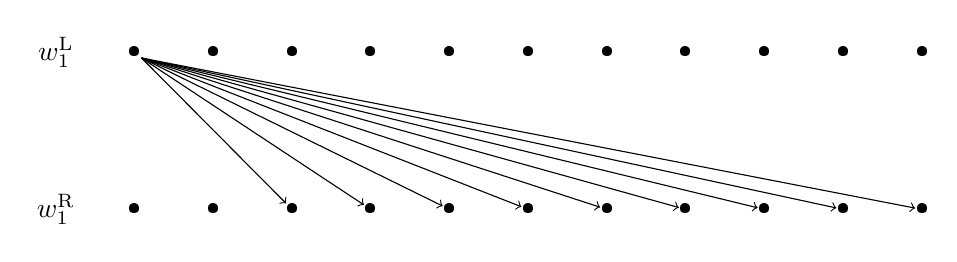
\begin{tikzpicture}
      \node at (-1,2) {$w_1^\textup{L}$};
      \node at (-1,0) {$w_1^\textup{R}$};
      \foreach \x in {0,...,10}
        \foreach \y in {0,...,1}
          \node[inner sep=0,outer sep=0] (n\y\x) at (\x,2*\y) {\textbullet};
      \foreach \x in {2,...,10}
        \draw[->] (n10.south east) -- (n0\x);
    \end{tikzpicture}
    \caption{No sparsification.}\label{fig:no_spars}
  \end{subfigure}
  \par\bigskip\bigskip
  \begin{subfigure}[ht]{\textwidth}
    \centering
    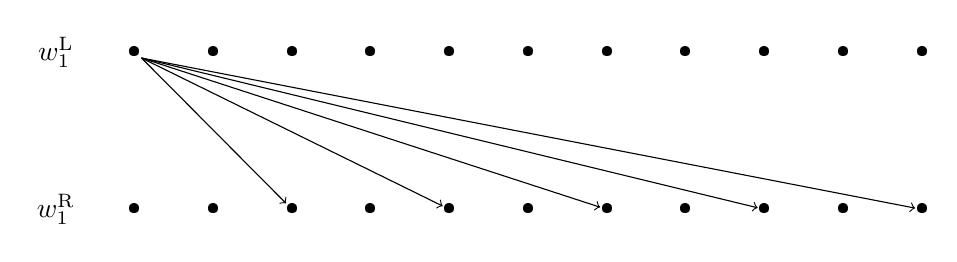
\begin{tikzpicture}
      \node at (-1,2) {$w_1^\textup{L}$};
      \node at (-1,0) {$w_1^\textup{R}$};
      \foreach \x in {0,...,10}
        \foreach \y in {0,...,1}
          \node[inner sep=0,outer sep=0] (n\y\x) at (\x,2*\y) {\textbullet};
      \foreach \x in {1,...,5}
        {\pgfmathtruncatemacro{\doublex}{\x * 2} \draw[->] (n10.south east) -- (n0\doublex);}
    \end{tikzpicture}
    \caption{Fixed step sparsification with $s = 2$.}\label{fig:fixed_spars}
  \end{subfigure}
  \par\bigskip\bigskip
  \begin{subfigure}[ht]{\textwidth}
    \centering
    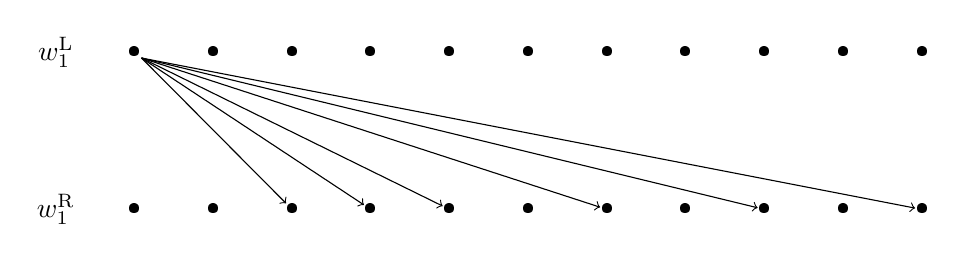
\begin{tikzpicture}
      \node at (-1,2) {$w_1^\textup{L}$};
      \node at (-1,0) {$w_1^\textup{R}$};
      \foreach \x in {0,...,10}
        \foreach \y in {0,...,1}
          \node[inner sep=0,outer sep=0] (n\y\x) at (\x,2*\y) {\textbullet};
      \foreach \x in {1,...,5}
        {\pgfmathtruncatemacro{\doublex}{\x * 2} \draw[->] (n10.south east) -- (n0\doublex);}
      \draw[->] (n10.south east) -- (n03);
    \end{tikzpicture}
    \caption{Fixed step sparsification with $s = 2$ and threshold $\tau = 3$.}\label{fig:threshold_spars}
  \end{subfigure}
  \par\bigskip\bigskip
  \begin{subfigure}[ht]{\textwidth}
    \centering
    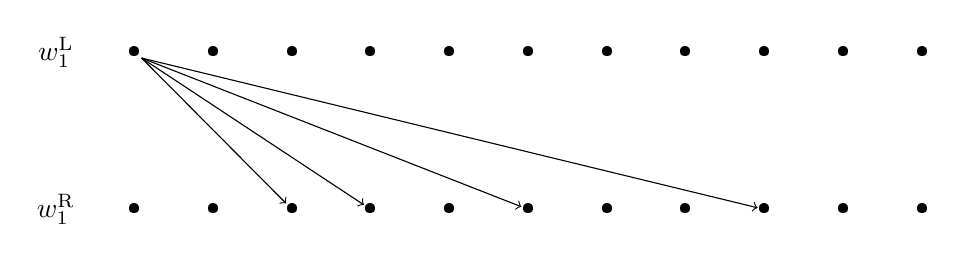
\begin{tikzpicture}
      \node at (-1,2) {$w_1^\textup{L}$};
      \node at (-1,0) {$w_1^\textup{R}$};
      \foreach \x in {0,...,10}
        \foreach \y in {0,...,1}
          \node[inner sep=0,outer sep=0] (n\y\x) at (\x,2*\y) {\textbullet};
      \draw[->] (n10.south east) -- (n02);
      \draw[->] (n10.south east) -- (n03);
      \draw[->] (n10.south east) -- (n05);
      \draw[->] (n10.south east) -- (n08);
    \end{tikzpicture}
    \caption{Progressive sparsification.}\label{fig:progressive_spars}
  \end{subfigure}
  \caption{Graphical representation of various graph sparsification techniques on the time-space graph.}\label{fig:spars}
\end{figure}

  \section{Computational Results}\label{sec:computational_results}

The aim of computational results presented in this section is to verify that the proposed approach is valid for complex instances coming from real-life applications, that describe an extended network with many trains, and an extended time horizon with a dense discretisation. We also want to validate that our algorithm achieves good results in real-time settings, where running times are limited to few seconds.

To this end, we have initially considered 23 instances, generated from three different real-world railway networks, provided to us by Alstom Transport. The first set of instances (N01-N13) describes a relatively small network chatacterised by the presence of single track lines used in both directions. The second set of six instances (L01-L06) refers to a busy regional network with a large main station and several smaller stations. Finally, the third set includes four instances (P01-P04) describing a high-speed network with frequent long-distance trains.

\Cref{tbl:instances_description} outlines the main characteristics of the instances considered. Column ``\# Trains'' lists the number of trains present in the instance; ``\# Nodes'' is the number of resources, i.e., the cardinality of the set $\Nodes$ in the network graph $\NetGraph$ (before time expansion); ``Time horizon'' is the span, in hours, of the planning horizon; ``Discretisation'' is the time discretisation step used, expressed in seconds; ``\# Conflicts'' is the sum of the number of conflicts (as described in \Cref{ssec:conflicts}: illegal overtaking, hard capacity violation, headway time violation) plus the number of violated mandatory time dependencies, given as input in the current train plan.

\begin{table}
    \begin{center}
        \begin{tabular}{lrrrrr}
            \textbf{Name} & \textbf{\# Trains} & \textbf{\# Nodes} & \textbf{Time horizon (h)} & \textbf{Discretisation (s)} & \textbf{\# Conflicts} \\
            \hline
            N01 & 28 & 108 & 2 & 15 & 24 \\
            N02 & 16 & 167 & 2 & 15 & 15 \\
            N03 & 28 & 172 & 2 & 15 & 36 \\
            N04 & 17 & 112 & 2 & 15 & 4 \\
            N05 & 18 & 112 & 2 & 15 & 12 \\
            N06 & 17 & 112 & 2 & 15 & 2 \\
            N07 & 28 & 126 & 2 & 15 & 12 \\
            N08 & 30 & 132 & 2 & 15 & 5 \\
            N09 & 28 & 130 & 2 & 15 & 4 \\
            N10 & 30 & 135 & 2 & 15 & 3 \\
            N11 & 15 & 137 & 1 & 15 & 1 \\
            N12 & 20 & 153 & 1 & 15 & 2 \\
            N13 & 33 & 135 & 4 & 15 & 37 \\
            L01 & 139 & 664 & 1 & 15 & 20 \\
            L02 & 103 & 631 & 0.75 & 15 & 54 \\
            L03 & 131 & 666 & 1 & 15 & 62 \\
            L04 & 132 & 675 & 1 & 15 & 25 \\
            L05 & 151 & 673 & 1.25 & 15 & 97 \\
            L06 & 133 & 671 & 1 & 15 & 38 \\
            P01 & 55 & 859 & 1 & 10 & 22 \\
            P02 & 55 & 814 & 1 & 10 & 22 \\
            P03 & 61 & 742 & 1 & 10 & 72 \\
            P04 & 71 & 731 & 1 & 10 & 70 \\
            \hline
        \end{tabular}
    \end{center}
    \caption{Main characteristics of the instances provided by Alstom.}\label{tbl:instances_description}
\end{table}

In \Cref{ssec:ptuning} we perform parameter tuning, to determine which graph sparsification methods and initial sortings are more likely to produce good solutions when used together with each policy (RVNS or Tabu) and time limit (2s or 10s). In \Cref{ssec:ptest} we run a simple parallel version of the algorithm on the 23 instances, using the tuned parameters.

In order to validate and benchmark our approach, we also generated new instances, which we are making publicly available. We used the network topology of the 2012 RAS Competition instances (see \citet{informs2012problem}), in two configurations: in the first (letter ``N''), each segment is modelled as a separate resource, giving an N-track scenario; in the second (letter ``S'') parallel tracks are not modelled separately, but as a single resource with the appropriate capacity, giving a single-track scenario. We generated 15 instances of each type, divided in groups of 3. The nominal timetable is the same for each group, while the disturbances change, so to have 5 different forecast timetables for each nominal one. Because the RAS network is smaller than the networks used in the instances of \Cref{tbl:instances_description}, in order to obtain feasible nominal timetables we had to either use fewer trains (instances of the first group), or a longer time horizon with a more coarse discretisation (instances of the second and third groups). These instances are available at \cite{alberto_santini_2017_322571}.

%\Cref{fig:ras_inst_micro} shows the network topology of the RAS instances in the more microscopic representation, while \Cref{fig:ras_inst_macro} shows the same network in the more macrospoic representations.
%\begin{sidewaysfigure}
  \begin{center}
    \resizebox{\textwidth}{!}{%
    \begin{tikzpicture}
      \node (n0) at (0,0) {\huge\textbullet};
      \node (n1) at (0.3,0) {\huge\textbullet};
      \node (n3) at (2.3,0) {\huge\textbullet};
      \node (n5) at (2.6,0) {\huge\textbullet};
      \node (n6) at (7.6,0) {\huge\textbullet};
      \node (n7) at (11.6,0) {\huge\textbullet};
      \node (n8) at (11.9,0) {\huge\textbullet};
      \node (n10) at (13.9,0) {\huge\textbullet};
      \node (n12) at (14.2,0) {\huge\textbullet};
      \node (n13) at (19.2,0) {\huge\textbullet};
      \node (n14) at (24.2,0) {\huge\textbullet};
      \node (n15) at (24.5,0) {\huge\textbullet};
      \node (n17) at (26.5,0) {\huge\textbullet};
      \node (n19) at (26.8,0) {\huge\textbullet};
      \node (n20) at (31.8,0) {\huge\textbullet};
      \node (n21) at (37.8,0) {\huge\textbullet};
      \node (n22) at (38.1,0) {\huge\textbullet};
      \node (n25) at (40.1,0) {\huge\textbullet};
      \node (n26) at (40.4,0) {\huge\textbullet};
      \node (n27) at (41.4,0) {\huge\textbullet};
      \node (n28) at (41.7,0) {\huge\textbullet};
      \node (n30) at (44.7,0) {\huge\textbullet};
      \node (n31) at (47.7,0) {\huge\textbullet};
      \node (n32) at (48,0) {\huge\textbullet};
      \node (n34) at (50,0) {\huge\textbullet};
      \node (n36) at (50.3,0) {\huge\textbullet};
      \node (n37) at (53.5,0) {\huge\textbullet};
      \node (n40) at (53.8,0) {\huge\textbullet};
      \node (n43) at (55.8,0) {\huge\textbullet};
      \node (n45) at (58.8,0) {\huge\textbullet};
      \node (n47) at (59.1,0) {\huge\textbullet};
      \node (n49) at (63.1,0) {\huge\textbullet};
      \node (n50) at (63.4,0) {\huge\textbullet};
      \node (n52) at (65.4,0) {\huge\textbullet};
      \node (n55) at (65.7,0) {\huge\textbullet};
      \node (n56) at (67.7,0) {\huge\textbullet};
      \node (n58) at (68,0) {\huge\textbullet};
      \node (n60) at (71,0) {\huge\textbullet};
      \node (n62) at (74,0) {\huge\textbullet};
      \node (n64) at (74.3,0) {\huge\textbullet};
      \node (n66) at (77.3,0) {\huge\textbullet};
      \node (n68) at (80.3,0) {\huge\textbullet};
      \node (n69) at (80.6,2) {\huge\textbullet};
      \node (n70) at (85.6,2) {\huge\textbullet};
      \node (n71) at (90.6,2) {\huge\textbullet};
      \node (n72) at (90.9,2) {\huge\textbullet};
      \node (n74) at (93.9,2) {\huge\textbullet};
      \node (n76) at (94.2,2) {\huge\textbullet};
      \node (n77) at (98.2,2) {\huge\textbullet};
      \node (n78) at (102.2,2) {\huge\textbullet};
      \node (n79) at (102.5,2) {\huge\textbullet};
      \node (n81) at (104.5,2) {\huge\textbullet};
      \node (n38) at (104.8,2) {\huge\textbullet};
      \node (n39) at (109.8,2) {\huge\textbullet};

      \node (n41) at (53.8,2) {\huge\textbullet};
      \node (n42) at (55.8,2) {\huge\textbullet};
      \node (n44) at (58.8,2) {\huge\textbullet};
      \node (n46) at (59.1,2) {\huge\textbullet};
      \node (n48) at (63.1,2) {\huge\textbullet};
      \node (n54) at (67.7,2) {\huge\textbullet};
      \node (n57) at (68,2) {\huge\textbullet};
      \node (n59) at (71,2) {\huge\textbullet};
      \node (n61) at (74,2) {\huge\textbullet};
      \node (n63) at (74.3,2) {\huge\textbullet};
      \node (n65) at (77.3,2) {\huge\textbullet};
      \node (n67) at (80.3,2) {\huge\textbullet};

      \node (n2) at (0.3,2) {\huge\textbullet};
      \node (n4) at (2.3,2) {\huge\textbullet};
      \node (n16) at (24.5,2) {\huge\textbullet};
      \node (n18) at (26.5,2) {\huge\textbullet};
      \node (n33) at (48,2) {\huge\textbullet};
      \node (n35) at (50,2) {\huge\textbullet};
      \node (n51) at (63.4,-2) {\huge\textbullet};
      \node (n53) at (65.4,-2) {\huge\textbullet};
      \node (n80) at (102.5,0) {\huge\textbullet};
      \node (n82) at (104.5,0) {\huge\textbullet};

      \draw[-] (n0.center) -- (n1.center) -- (n3.center) -- (n5.center) -- (n6.center) -- (n7.center) -- (n8.center) -- (n10.center) -- (n12.center) -- (n13.center) -- (n14.center) -- (n15.center) -- (n17.center) -- (n19.center);
      \draw[-] (n19.center) -- (n20.center) -- (n21.center) -- (n22.center) -- (n25.center) -- (n26.center) -- (n27.center) -- (n28.center) -- (n30.center) -- (n31.center) -- (n32.center) -- (n34.center) -- (n36.center);
      \draw[-] (n36.center) -- (n37.center) -- (n40.center) -- (n43.center) -- (n45.center) -- (n47.center) -- (n49.center) -- (n50.center) -- (n52.center) -- (n55.center) -- (n56.center) -- (n58.center) -- (n60.center);
      \draw[-] (n60.center) -- (n62.center) -- (n64.center) -- (n66.center) -- (n68.center) -- (n69.center) -- (n70.center) -- (n71.center) -- (n72.center) -- (n74.center) -- (n76.center) -- (n77.center) -- (n78.center);
      \draw[-] (n78.center) -- (n79.center) -- (n81.center) -- (n38.center) -- (n39.center);
      \draw[-] (n37.center) -- (n41.center) -- (n42.center) -- (n44.center) -- (n46.center) -- (n48.center) -- (n54.center) -- (n57.center) -- (n59.center) -- (n61.center) -- (n63.center) -- (n65.center) -- (n67.center) -- (n69.center);
      \draw[-] (n0.center) -- (n2.center) -- (n4.center) -- (n5.center);
      \draw[-] (n14.center) -- (n16.center) -- (n18.center) -- (n19.center);
      \draw[-] (n31.center) -- (n33.center) -- (n35.center) -- (n36.center);
      \draw[-] (n49.center) -- (n51.center) -- (n53.center) -- (n55.center);
      \draw[-] (n78.center) -- (n80.center) -- (n82.center) -- (n38.center);
      \draw[-] (n45.center) -- (n46.center);
      \draw[-] (n44.center) -- (n47.center);
      \draw[-] (n54.center) -- (n58.center);
      \draw[-] (n56.center) -- (n57.center);
    \end{tikzpicture}}
    \caption{Network topology of the RAS-based instances. In this representation, each track is modelled separately.}\label{fig:ras_inst_micro}
    \vspace{1em}
    \resizebox{\textwidth}{!}{%
    \begin{tikzpicture}
      \node (n0) at (0,0) {\huge\textbullet};
      \node (n1) at (0.3,0) {\huge\textbullet};
      \node (n3) at (2.3,0) {\huge\textbullet};
      \node (n5) at (2.6,0) {\huge\textbullet};
      \node (n6) at (7.6,0) {\huge\textbullet};
      \node (n7) at (11.6,0) {\huge\textbullet};
      \node (n8) at (11.9,0) {\huge\textbullet};
      \node (n10) at (13.9,0) {\huge\textbullet};
      \node (n12) at (14.2,0) {\huge\textbullet};
      \node (n13) at (19.2,0) {\huge\textbullet};
      \node (n14) at (24.2,0) {\huge\textbullet};
      \node (n15) at (24.5,0) {\huge\textbullet};
      \node (n17) at (26.5,0) {\huge\textbullet};
      \node (n19) at (26.8,0) {\huge\textbullet};
      \node (n20) at (31.8,0) {\huge\textbullet};
      \node (n21) at (37.8,0) {\huge\textbullet};
      \node (n22) at (38.1,0) {\huge\textbullet};
      \node (n25) at (40.1,0) {\huge\textbullet};
      \node (n26) at (40.4,0) {\huge\textbullet};
      \node (n27) at (41.4,0) {\huge\textbullet};
      \node (n28) at (41.7,0) {\huge\textbullet};
      \node (n30) at (44.7,0) {\huge\textbullet};
      \node (n31) at (47.7,0) {\huge\textbullet};
      \node (n32) at (48,0) {\huge\textbullet};
      \node (n34) at (50,0) {\huge\textbullet};
      \node (n36) at (50.3,0) {\huge\textbullet};
      \node (n37) at (53.5,0) {\huge\textbullet};
      \node (n40) at (53.8,0) {\huge\textbullet};
      \node (n43) at (55.8,0) {\huge\textbullet};
      \node (n45) at (58.8,0) {\huge\textbullet};
      \node (n47) at (59.1,0) {\huge\textbullet};
      \node (n49) at (63.1,0) {\huge\textbullet};
      \node (n50) at (63.4,0) {\huge\textbullet};
      \node (n52) at (65.4,0) {\huge\textbullet};
      \node (n55) at (65.7,0) {\huge\textbullet};
      \node (n56) at (67.7,0) {\huge\textbullet};
      \node (n58) at (68,0) {\huge\textbullet};
      \node (n60) at (71,0) {\huge\textbullet};
      \node (n62) at (74,0) {\huge\textbullet};
      \node (n64) at (74.3,0) {\huge\textbullet};
      \node (n66) at (77.3,0) {\huge\textbullet};
      \node (n68) at (80.3,0) {\huge\textbullet};
      \node (n69) at (80.6,0) {\huge\textbullet};
      \node (n70) at (85.6,0) {\huge\textbullet};
      \node (n71) at (90.6,0) {\huge\textbullet};
      \node (n72) at (90.9,0) {\huge\textbullet};
      \node (n74) at (93.9,0) {\huge\textbullet};
      \node (n76) at (94.2,0) {\huge\textbullet};
      \node (n77) at (98.2,0) {\huge\textbullet};
      \node (n78) at (102.2,0) {\huge\textbullet};
      \node (n79) at (102.5,0) {\huge\textbullet};
      \node (n81) at (104.5,0) {\huge\textbullet};
      \node (n38) at (104.8,0) {\huge\textbullet};
      \node (n39) at (109.8,0) {\huge\textbullet};
      \draw[-] (n0.center) -- (n1.center) -- (n3.center) -- (n5.center) -- (n6.center) -- (n7.center) -- (n8.center) -- (n10.center) -- (n12.center) -- (n13.center) -- (n14.center) -- (n15.center) -- (n17.center) -- (n19.center);
      \draw[-] (n19.center) -- (n20.center) -- (n21.center) -- (n22.center) -- (n25.center) -- (n26.center) -- (n27.center) -- (n28.center) -- (n30.center) -- (n31.center) -- (n32.center) -- (n34.center) -- (n36.center);
      \draw[-] (n36.center) -- (n37.center) -- (n40.center) -- (n43.center) -- (n45.center) -- (n47.center) -- (n49.center) -- (n50.center) -- (n52.center) -- (n55.center) -- (n56.center) -- (n58.center) -- (n60.center);
      \draw[-] (n60.center) -- (n62.center) -- (n64.center) -- (n66.center) -- (n68.center) -- (n69.center) -- (n70.center) -- (n71.center) -- (n72.center) -- (n74.center) -- (n76.center) -- (n77.center) -- (n78.center);
      \draw[-] (n78.center) -- (n79.center) -- (n81.center) -- (n38.center) -- (n39.center);
    \end{tikzpicture}}
  \end{center}
  \caption{Network topology of the RAS-based instances. In this representation, each set of parallel tracks is modelled as one single resource.}\label{fig:ras_inst_macro}
\end{sidewaysfigure}


To ease the comparison with other algorithms that might be developped in the future, we did not consider problem-specific features such as time dependencies, and splits and merges. The conflicts that can arise, therefore, are limited to headway, hard and soft capacity, crossing, and overtake violations. Soft violations are penalised with a simple linear function. \Cref{tbl:ras_instances_description} describes the features of the generated instances; columns ``H'', ``O'', and ``C'' give a detailed breakdown of the type of conflicts: headways, overtake, and hard capacity, respectively. In \Cref{ssec:ptest} we apply the tuned parallel algorithm to the new instances, similarly to what we do for the proprietary instances.

\begin{table}
  \begin{center}
    \begin{tabular}{lrrrrrr}
      & & & & \multicolumn{3}{c}{\textbf{\# Conflicts}} \\
      \textbf{Name} & \textbf{\# Trains} & \textbf{Time horizon (h)} & \textbf{Discretisation (s)} & \textbf{H} & \textbf{O} & \textbf{C} \\
      \hline
      N-1-1 & 7  & 4  & 15 & 0 & 0 & 6 \\
      N-1-2 & 7  & 4  & 15 & 63 & 0 & 43 \\
      N-1-3 & 7  & 4  & 15 & 35 & 2 & 41 \\
      N-1-4 & 7  & 4  & 15 & 35 & 1 & 42 \\
      N-1-5 & 7  & 4  & 15 & 0 & 0 & 32 \\
      N-2-1 & 12 & 12 & 60 & 2 & 0 & 3 \\
      N-2-2 & 12 & 12 & 60 & 4 & 0 & 6 \\
      N-2-3 & 12 & 12 & 60 & 2 & 0 & 4 \\
      N-2-4 & 12 & 12 & 60 & 0 & 0 & 7 \\
      N-2-5 & 12 & 12 & 60 & 6 & 0 & 13 \\
      N-3-1 & 24 & 12 & 60 & 4 & 0 & 25 \\
      N-3-2 & 24 & 12 & 60 & 105 & 0 & 53 \\
      N-3-3 & 24 & 12 & 60 & 0 & 0 & 6 \\
      N-3-4 & 24 & 12 & 60 & 103 & 0 & 89 \\
      N-3-5 & 24 & 12 & 60 & 0 & 0 & 10 \\
      S-1-1 & 7  & 4  & 15 & 0 & 0 & 3 \\
      S-1-2 & 7  & 4  & 15 & 32 & 0 & 22 \\
      S-1-3 & 7  & 4  & 15 & 4 & 1 & 28 \\
      S-1-4 & 7  & 4  & 15 & 30 & 1 & 24 \\
      S-1-5 & 7  & 4  & 15 & 2 & 0 & 19 \\
      S-2-1 & 12 & 12 & 60 & 0 & 0 & 2 \\
      S-2-2 & 12 & 12 & 60 & 2 & 0 & 2 \\
      S-2-3 & 12 & 12 & 60 & 6 & 0 & 5 \\
      S-2-4 & 12 & 12 & 60 & 0 & 0 & 4 \\
      S-2-5 & 12 & 12 & 60 & 2 & 0 & 4 \\
      S-3-1 & 24 & 12 & 60 & 0 & 0 & 21 \\
      S-3-2 & 24 & 12 & 60 & 59 & 0 & 25 \\
      S-3-3 & 24 & 12 & 60 & 0 & 0 & 4 \\
      S-3-4 & 24 & 12 & 60 & 60 & 0 & 60 \\
      S-3-5 & 24 & 12 & 60 & 2 & 0 & 12 \\
      \hline
    \end{tabular}
    \caption{Main characteristics of the instances generated starting from the 2012 RAS Competition instances.}\label{tbl:ras_instances_description}
  \end{center}
\end{table}

The tests presented in this section have been run on a dual-core 3.2GHz Intel i5 machine, with 7803MB of RAM. The CPU configuration and the L1, L2 and L3 cache sizes are detailed in \Cref{fig:cputopo}, as produced by the software Hwloc (\citet{Broquedis2010}).

\begin{figure}
  \begin{center}
    \includegraphics[width=0.33\textwidth]{figures/cputopo.png}
  \end{center}
  \caption{Schematic hardware configuration of the test machine.}\label{fig:cputopo}
\end{figure}

\subsection{Parameter tuning}\label{ssec:ptuning}

The objective of parameter tuning is to measure the impact of the sparsification methods and the sorting criteria introduced in \Cref{sec:solution_algorithm}, on real-time applications of the algorithm.

We ran six sets of experiments overall, in order to determine which combinations of sparsification and sorting are particularly effective with the RVNS and Tabu policies. For each of these two policies, the three sets of experiments only vary in the hard time limit given to the algorithm. The first two time limits are of 2 and 10 seconds (real-time); the third time limit is of 60 seconds, and is used to provide better solutions that can be used as a baseline for comparisons.

For each set of experiments, the tests were run on all the 23 Alstom instances. For each instance, we tried all combinations of sparsification methods and initial sortings, using the parameters described in \Cref{sec:solution_algorithm}. In total, we had 19 possible settings for the sparsification methods and 7 possible sortings, giving 133 tests for each policy, time limit and instance, giving a grand total of $133 \cdot 2 \cdot 3 \cdot 23 = 18\;\!354$ runs.

\begin{sidewaystable}\footnotesize
    \begin{center}
        \begin{tabular}{lrrrrrrrrrrrr}
            & \multicolumn{3}{c}{\textbf{Tabu 2s}} & \multicolumn{3}{c}{\textbf{Tabu 10s}} & \multicolumn{3}{c}{\textbf{RVNS 2s}} & \multicolumn{3}{c}{\textbf{RVNS 10s}} \\
            \cmidrule(lr){2-4}\cmidrule{5-7}\cmidrule(lr){8-10}\cmidrule(lr){11-13}
            \textbf{Sparsification} &
            \textbf{CF} & \textbf{Dev} & \textbf{CF Dev} &
            \textbf{CF} & \textbf{Dev} & \textbf{CF Dev} &
            \textbf{CF} & \textbf{Dev} & \textbf{CF Dev} &
            \textbf{CF} & \textbf{Dev} & \textbf{CF Dev} \\
            \cmidrule(lr){1-1}\cmidrule(lr){2-4}\cmidrule{5-7}\cmidrule(lr){8-10}\cmidrule(lr){11-13}
            disabled       & 0.64 & 10912.64 & 1.88 & 0.78 & 593.90   & 1.33 & 0.79 & 488.43   & 10.32 & 0.80 & 370.22   & 1.43 \\
            fixed-2        & 0.70 & 16252.12 & 1.68 & 0.77 & 15374.42 & 1.35 & 0.75 & 15811.52 & 1.73  & 0.75 & 15558.96 & 1.38 \\
            fixed-3        & 0.71 & 16161.95 & 1.66 & 0.78 & 15312.86 & 1.34 & 0.75 & 15686.94 & 1.62  & 0.76 & 15528.27 & 1.42 \\
            fixed-5        & 0.74 & 15875.32 & 1.62 & 0.78 & 15321.86 & 1.32 & 0.74 & 28820.40 & 1.59  & 0.75 & 26406.56 & 1.40 \\
            linear-2       & 0.65 & 6391.54  & 1.85 & 0.80 & 339.41   & 1.36 & 0.80 & 377.08   & 10.06 & 0.80 & 370.23   & 1.45 \\
            linear-3       & 0.64 & 8725.04  & 2.06 & 0.78 & 418.67   & 1.39 & 0.79 & 599.52   & 10.20 & 0.80 & 370.24   & 1.46 \\
            linear-5       & 0.62 & 11325.47 & 1.95 & 0.77 & 739.40   & 1.43 & 0.78 & 4981.04  & 8.29  & 0.80 & 370.25   & 1.47 \\
            progressive-2  & 0.76 & 834.95   & 1.49 & 0.82 & 31.93    & 1.24 & 0.78 & 696.63   & 1.51  & 0.80 & 308.66   & 1.34 \\
            progressive-3  & 0.73 & 1348.76  & 1.41 & 0.81 & 62.66    & 1.23 & 0.80 & 493.27   & 1.55  & 0.80 & 247.19   & 1.34 \\
            progressive-5  & 0.73 & 1439.36  & 1.50 & 0.82 & 64.21    & 1.23 & 0.78 & 663.47   & 1.57  & 0.78 & 379.93   & 1.32 \\
            threshold-2-5  & 0.66 & 3977.49  & 4.29 & 0.80 & 217.94   & 1.26 & 0.80 & 406.13   & 7.95  & 0.80 & 370.16   & 1.38 \\
            threshold-2-10 & 0.67 & 3851.51  & 4.25 & 0.79 & 247.15   & 1.27 & 0.78 & 445.13   & 8.05  & 0.79 & 339.43   & 1.38 \\
            threshold-2-15 & 0.66 & 4157.31  & 4.34 & 0.79 & 310.16   & 1.27 & 0.80 & 406.14   & 7.95  & 0.80 & 370.17   & 1.38 \\
            threshold-3-5  & 0.70 & 1482.97  & 1.62 & 0.80 & 247.14   & 1.28 & 0.79 & 568.01   & 7.93  & 0.80 & 370.15   & 1.36 \\
            threshold-3-10 & 0.69 & 1627.55  & 1.63 & 0.80 & 247.15   & 1.29 & 0.78 & 475.82   & 7.99  & 0.79 & 400.89   & 1.36 \\
            threshold-3-15 & 0.68 & 1742.63  & 4.20 & 0.80 & 187.18   & 1.24 & 0.79 & 436.84   & 7.95  & 0.79 & 370.16   & 1.36 \\
            threshold-5-5  & 0.73 & 1333.08  & 1.49 & 0.81 & 93.41    & 1.22 & 0.79 & 556.38   & 3.63  & 0.79 & 308.66   & 1.34 \\
            threshold-5-10 & 0.70 & 1708.34  & 1.56 & 0.81 & 93.42    & 1.24 & 0.79 & 525.67   & 3.67  & 0.79 & 370.14   & 1.34 \\
            threshold-5-15 & 0.69 & 1750.12  & 1.58 & 0.81 & 62.70    & 1.27 & 0.79 & 525.69   & 3.69  & 0.79 & 400.89   & 1.36 \\
            \cmidrule(lr){1-1}\cmidrule(lr){2-4}\cmidrule{5-7}\cmidrule(lr){8-10}\cmidrule(lr){11-13}
        \end{tabular}
    \end{center}
    \caption{Parameter tuning results aggregated by sparsification method.}\label{tbl:par_tun_results_spars}
\end{sidewaystable}

\begin{sidewaystable}\footnotesize
    \begin{center}
        \begin{tabular}{lrrrrrrrrrrrr}
            & \multicolumn{3}{c}{\textbf{Tabu 2s}} & \multicolumn{3}{c}{\textbf{Tabu 10s}} & \multicolumn{3}{c}{\textbf{RVNS 2s}} & \multicolumn{3}{c}{\textbf{RVNS 10s}} \\
            \cmidrule(lr){2-4}\cmidrule{5-7}\cmidrule(lr){8-10}\cmidrule(lr){11-13}
            \textbf{Sorting} &
            \textbf{CF} & \textbf{Dev} & \textbf{CF Dev} &
            \textbf{CF} & \textbf{Dev} & \textbf{CF Dev} &
            \textbf{CF} & \textbf{Dev} & \textbf{CF Dev} &
            \textbf{CF} & \textbf{Dev} & \textbf{CF Dev} \\
            \cmidrule(lr){1-1}\cmidrule(lr){2-4}\cmidrule{5-7}\cmidrule(lr){8-10}\cmidrule(lr){11-13}
            Congestion         & 0.73 & 3197.61  & 1.58 & 0.80 & 2509.98 & 1.29 & 0.79 & 3535.41 & 11.38  & 0.80 & 3349.47 & 1.42 \\
            Conflict time      & 0.73 & 7938.66  & 4.92 & 0.80 & 2589.95 & 1.28 & 0.78 & 4012.83 & 9.14   & 0.78 & 3700.91 & 1.31 \\
            Length             & 0.73 & 3302.75  & 1.64 & 0.80 & 2635.49 & 1.27 & 0.78 & 3882.08 & 1.75   & 0.78 & 3791.12 & 1.44 \\
            Random             & 0.59 & 13031.87 & 2.01 & 0.81 & 2637.88 & 1.34 & 0.76 & 5482.95 & 9.27   & 0.78 & 2623.51 & 1.45 \\
            Reverse congestion & 0.74 & 5170.65  & 1.72 & 0.78 & 2589.07 & 1.29 & 0.78 & 3848.59 & 1.77   & 0.78 & 3756.94 & 1.37 \\
            Reverse speed      & 0.65 & 4110.60  & 1.61 & 0.79 & 2584.59 & 1.26 & 0.77 & 2890.27 & 1.75   & 0.77 & 2841.63 & 1.35 \\
            Speed              & 0.68 & 4105.06  & 1.70 & 0.79 & 2861.43 & 1.31 & 0.82 & 3229.39 & 4.74   & 0.82 & 3224.74 & 1.33 \\
            \cmidrule(lr){1-1}\cmidrule(lr){2-4}\cmidrule{5-7}\cmidrule(lr){8-10}\cmidrule(lr){11-13}
        \end{tabular}
    \end{center}
    \caption{Parameter tuning results aggregated by initial sorting.}\label{tbl:par_tun_results_sort}
\end{sidewaystable}

\Cref{tbl:par_tun_results_spars} and \Cref{tbl:par_tun_results_sort} show the results we obtained during parameter tuning for the two solvers, with time limits 2 and 10 seconds. In the first table the results have been aggregated by sparsification method, while in the second, they have been aggregated by sorting criterion.

Columns ``Sparsification'' (in \Cref{tbl:par_tun_results_spars}) or ``Sorting'' (in \Cref{tbl:par_tun_results_sort}) tell, respectively, for which sparsification method or sorting criterion the data is being aggregated. For each line the data are grouped in four blocks, corresponding to the four combinations of policy (Tabu or RVNS) and time limit (2s or 10s). Column ``CF'' gives the fraction of tests for which the algorithm was able to find a conflict-free schedule. Column ``Dev'' is the average deviation, calculated as $(z - z^*) / z^*$ where $z$ is the solution value obtained by the algorithm with the specified configuration, and $z^*$ is the best known solution value. This best known value comes from the 60 seconds runs that we use as baseline, and is the best value across all possible parameter combinations. Since, as explained in \Cref{sec:solution_algorithm}, the objective function has a hierarchical structure and unresolved conflicts take a very large penalty, the values in this column tend to be quite large, as one single instance for which a method was not able to produce a conflict-free schedule can increase the average considerably. This is, however, a good metric of the desirability of a method, because solving conflicts always has priority on any other measure of solution quality. In column ``CF Dev'', we similarly report the average deviation, but this time we only consider the conflict-free solutions in the average.

We want to select the best sparsification method for each policy (RVNS or Tabu) and each time limit (2s or 10s). In order to do this, it is not sufficient to take the policy with the lowest deviation, but one has to ensure that the differences in deviation are statistically relevant.

For this reason, we ran a Wilcoxon signed-rank test on each pair of sparsification methods, to measure whether their deviations across the various instances come from the same distribution or not (in this latter case, a difference in the average deviation is statistically relevant).

\begin{figure}
    \begin{subfigure}[ht]{0.5\textwidth}
        \begin{center}
            \includegraphics[width=0.95\textwidth]{figures/spars-2-tabu.png}
        \end{center}
        \caption{Policy: Tabu, time limit: 2s.}\label{sfig:wilcoxon_2_tabu}
    \end{subfigure}
    \begin{subfigure}[ht]{0.5\textwidth}
        \begin{center}
            \includegraphics[width=0.75\textwidth]{figures/spars-2-vns.png}
        \end{center}
        \caption{Policy: RVNS, time limit: 2s.}\label{sfig:wilcoxon_2_vns}
    \end{subfigure}
    \caption{Visual representation of the results of the Wilcoxon test (time limit: 2s).}\label{fig:wilcoxon_2}
\end{figure}

\begin{figure}
    \begin{subfigure}[ht]{\textwidth}
        \begin{center}
            \includegraphics[width=0.95\textwidth]{figures/spars-10-tabu.png}
        \end{center}
        \caption{Policy: Tabu, time limit: 10s.}\label{sfig:wilcoxon_10_tabu}
    \end{subfigure}
    \par\bigskip
    \begin{subfigure}[ht]{\textwidth}
        \begin{center}
            \includegraphics[width=0.75\textwidth]{figures/spars-10-vns.png}
        \end{center}
        \caption{Policy: RVNS, time limit: 10s.}\label{sfig:wilcoxon_10_vns}
    \end{subfigure}
    \caption{Visual representation of the results of the Wilcoxon test (time limit: 10s).}\label{fig:wilcoxon_10}
\end{figure}

\Cref{fig:wilcoxon_2} and \Cref{fig:wilcoxon_10} give a graphical representation of the outcomes of the Wilcoxon test. Each figure gives a representation of a directed graph. Sparsification methods are represented as nodes. An arc is drawn between two nodes if the $p$-value of the Wilcoxon test relative to two sparsifications is $<0.05$; the arc goes from the node with the better average deviation to that with the worse one. The colour and the thickness of the arc depend on the difference between the deviations: the greater the difference, the thicker and bluer the arc; on the other hand, small differences are represented by thin red-ish arcs. In particular, notice that the thickness and colour of the arc are not related with the $p$-value, which is used only as a threshold to decide whether to create the arc.

To simplify the visualisation, nodes and arcs are drawn from top to bottom, so that the best sparsifications are in the top part of the graph. Furthemore, in order to reduce the number of arcs drawn in the figure, whenever there are arcs $(M_1, M_2), (M_2, M_3)$ and $(M_1, M_3)$, this latter arc is removed. In other terms, if a method $M_1$ dominates method $M_2$, and $M_2$ dominates $M_3$, it is implicit that $M_1$ dominates $M_3$.

The sparisification methods were chosen as follows:
\begin{itemize}
    \item In the case of policy Tabu and time limit 2s (\Cref{sfig:wilcoxon_2_tabu}) the only two undominated methods are ``progressive-2'' and ``progressive-3''; since the average deviation of the former is 38.1\% smaller than that of the latter (see \Cref{tbl:par_tun_results_spars}), we decided to take ``progressive-2'' as the chosen sparsification method.
    \item For policy RVNS and time limit 2s, the only undominated method is ``linear-2'', which also has a considerably smaller deviation compared to the other methods.
    \item An interesting case is that of policy Tabu and time limit 10s (\Cref{sfig:wilcoxon_10_tabu}), as this is the case where it is most unclear which sparsification emerges as a winner. However, since the deviation of method ``progressive-2'' is the smallest, and it is 49.04\% smaller than the second-smallest one (``progressive-3''), we chose this method.
    \item Finally, for policy RVNS and time limit 10s, the three undominated methods were ``progressive-2'', ``progressive-3'', and ``threshold-5-5''. Again, since the average deviation for ``progressive-3'' is 19.92\% smaller than that for the other two (which have the same deviation), we chose that method.
\end{itemize}

\begin{table}\footnotesize%
	\tabcolsep=5pt
    \begin{center}
        \begin{tabular}{lrrrrrrrrrrrr}
            & \multicolumn{3}{c}{\textbf{Tabu 2s}} & \multicolumn{3}{c}{\textbf{Tabu 10s}} & \multicolumn{3}{c}{\textbf{RVNS 2s}}  & \multicolumn{3}{c}{\textbf{RVNS 10s}} \\
            & \multicolumn{3}{c}{\textbf{progressive-2}} & \multicolumn{3}{c}{\textbf{progressive-2}} & \multicolumn{3}{c}{\textbf{linear-2}} & \multicolumn{3}{c}{\textbf{progressive-3}} \\
            \cmidrule(lr){2-4}\cmidrule(lr){5-7}\cmidrule(lr){8-10}\cmidrule(lr){11-13}
            & \multicolumn{2}{c}{Deviation} & & \multicolumn{2}{c}{Deviation} & & \multicolumn{2}{c}{Deviation} & & \multicolumn{2}{c}{Deviation} & \\
			\cmidrule(lr){2-3}\cmidrule(lr){5-6}\cmidrule(lr){8-9}\cmidrule(lr){11-12}
			\textbf{Sorting} & Avg & Std & Best & Avg & Std & Best & Avg & Std & Best & Avg & Std & Best \\
            \cmidrule(lr){1-1}\cmidrule(lr){2-4}\cmidrule(lr){5-7}\cmidrule(lr){8-10}\cmidrule(lr){11-13}
            Congestion         & 441.45   & 2115.65 & 8 & 0.16   & 0.22    & 12 & 11.83  & 53.76   & 6 &   0.36 & 0.83    & 8 \\
            Conflict time      & 430.66   & 2063.77 & 2 & 0.22   & 0.30    &  2 & 442.05 & 2062.05 & 6 & 430.57 & 2063.81 & 5 \\
            Length             & 1076.20  & 5159.38 & 4 & 0.24   & 0.38    &  2 & 861.38 & 4127.40 & 2 & 215.53 & 1031.94 & 1 \\
            Random             & 2461.98  & 9855.31 & 3 & 0.22   & 0.31    &  2 & 227.90 & 1030.85 & 1 & 430.60 & 2063.80 & 3 \\
            Rev. Congestion    & 226.44   & 1083.85 & 3 & 0.14   & 0.16    &  2 & 646.11 & 3095.51 & 3 & 430.59 & 2063.73 & 1 \\
            Rev. Speed         & 554.88   & 1887.01 & 1 & 0.19   & 0.33    &  2 & 431.11 & 2063.69 & 3 & 215.47 & 1032.00 & 1 \\
            Speed              & 646.03   & 3095.86 & 2 & 215.37 & 1031.95 &  3 & 12.15  & 53.70   & 2 &   0.23 & 0.42    & 4 \\
            \cmidrule(lr){1-1}\cmidrule(lr){2-4}\cmidrule(lr){5-7}\cmidrule(lr){8-10}\cmidrule(lr){11-13}
        \end{tabular}
    \end{center}
    \caption{Average deviations of different sortings, for the chosen sparsification methods.}\label{tbl:chosen_spars}
\end{table}

\Cref{tbl:chosen_spars} shows the chosen sparsification methods and gives the average deviations (columns ``Avg''), together with their standard deviation (column ``Std''), obtained by employing the different initial sortings with each sparsification. Column ``Best'' tells the number of instances (out of 23) for which each sorting criterion provided the best result, compared to the other criteria in the same column.

\subsection{Parallel algorithm}\label{ssec:ptest}

\begin{table}
    \begin{center}
        \begin{tabular}{llll}
            \textbf{Tabu 2s} & \textbf{Tabu 10s} & \textbf{RVNS 2s} & \textbf{RVNS 10s} \\
            \textbf{progressive-2} & \textbf{progressive-2} & \textbf{linear-2} & \textbf{progressive-3} \\
            \hline
            \rule{0pt}{2.5ex}Congestion & Congestion & Congestion & Congestion \\
            Length & Conflict Time & Conflict Time & Conflict Time \\
            Reverse Congestion & Reverse Congestion & Reverse Congestion & Speed \\
            Random & Reverse Speed & Reverse Speed & Random \\
            \hline
        \end{tabular}
    \end{center}
    \caption{List of sorting criteria chosen for each policy and time limit, to be used in the parallel algorithm.}\label{tbl:chosen_sorts}
\end{table}

In this section we provide computational results for a very simple parallel implementation of the algorithm. We ran four sets of experiments, namely one for each combination of policy and time limit, together with the respective sparsification method chosen during parameter tuning, as described in \Cref{ssec:ptuning}. For each set, the parallel implementation simply consists of launching four parallel instances of the algorithm, each using one of four sorting criteria. When the time limit hits, the four solutions provided by the parallel instances are examined and the best one is returned as the overall solution.

The usage of parallel algorithms in operational research is well-established. We refer the reader to, e.g., \citet{clausen1999best} for parallel strategies for branch-and-bound exact algorithms, or to \citet{ropke2017palns} for a systematic analysis of the speed-ups obtained by parallelising the Adaptive Large Neighbourhood Search metaheuristic. With respect to the train rescheduling problem, \citet{iqbal2012parallel,iqbal2013multi} proposed parallel algorithms for rescheduling under disturbances.

In our case, the implementation of a parallel algorithm is motivated by the high dispersion of the solution values with respect to the average one, obtained by the different sorting methods, as witnessed by the high values of Standard Deviation reported in \Cref{tbl:chosen_spars} (this effect is more evident for the 2s time limit compared to the 10s one, and for the RVNS policy compared to the Tabu one). This means that, in practice, even the best sorting method was not able to resolve some solvable conflict, thus resulting in high solution values, due to the hierarchical nature of our objective function. Furthermore, we observed a certain complementarity in the capability of resolving conflicts across different sortings, which we see as a hint towards the parallel use of different sorting criteria.

More formally, we investigated the dependance of sorting criteria to instance characteristics via simple \emph{one-vs-all} and \emph{one-vs-one} multiclass classification algorithms provided by the library \texttt{scikit} (see, e.g., \citet{aly2005class}). These algorithms were based on the binary classifier that, for a fixed time limit, assigns an instance to an intial sorting criterion (class) if there is at least one policy (either Tabu or RVNS) for which that sorting provided the best result for that time limit. The instance features considered were the one listed in \Cref{tbl:instances_description,tbl:ras_instances_description}. Neither the \emph{one-vs-all} nor the \emph{one-vs-one} algorithm found statistically significant relationships of the sorting criteria to the instance features.

Once established the need for an algorithm that employs more than one sorting criteria at once, it is clearly important to perform a good choice of the criteria. The simplest approach would be to choose the four criteria that produce the four lowest deviations for a given policy and time limit (see \Cref{tbl:chosen_spars}). This choice, however, has not proven particularly good especially for the lowest time limit, and in one case we even had one instance (instance ``P4'' for the Tabu policy at 2s) for which not all solvable conflicts were actually resolved.

What we aim for is a choice of methods out of which, given any instance, there are high chances to find one that works reasonably well with that instance, eliminating all solvable conflicts, and therefore exploting the aforementioned complementarity. For this reason, we decided to choose the methods in a way to maximise the number of instances for which at least one of the methods chosen was the best. \Cref{tbl:chosen_sorts} lists the chosen sorting criterian for each policy and time limit.

\begin{table}\footnotesize
    \begin{center}
        \begin{tabular}{lllrrrrr}
            \textbf{Instance group} & \textbf{Algorithm} & \textbf{Sorting} & \textbf{Dev} & \textbf{Conflicts} & \textbf{Infeasible} & \textbf{Modified} & \textbf{Delay} \\
            \hline
            L   & Tabu 2s	& Random, Length, Reverse congestion    & 0.17  & 0.50 & 0.00 & 104.50 & 28.64 \\
            L   & Tabu 10s  & Reverse congestion                    & 0.11  & 0.50 & 0.00 & 104.67 & 29.00 \\
            L   & RVNS 2s	& Reverse speed                         & 0.17  & 0.50 & 0.00 & 105.67 & 33.34 \\
            L   & RVNS 10s  & Conflict time                         & 0.05  & 0.50 & 0.00 & 100.83 & 10.64 \\
            N   & Tabu 2s   & Congestion                            & 0.16  & 0.38 & 0.08 & 7.85   & 79.43 \\
            N   & Tabu 10s  & Congestion                            & 0.08  & 0.38 & 0.08 & 8.23   & 70.12 \\
            N   & RVNS 2s   & Congestion                            & 0.45  & 0.38 & 0.08 & 7.54   & 99.30 \\
            N   & RVNS 10s  & Congestion                            & 0.26  & 0.38 & 0.08 & 8.00   & 67.69 \\
            P   & Tabu 2s   & Reverse congestion                    & 0.50  & 0.00 & 0.00 & 59.25  & 247.17 \\
            P   & Tabu 10s  & Reverse speed                         & 0.03  & 0.00 & 0.00 & 59.50  & 220.52 \\
            P   & RVNS 2s   & Conflict time                         & 0.30  & 0.00 & 0.00 & 59.50  & 226.83 \\
            P   & RVNS 10s  & Congestion                            & 0.20  & 0.00 & 0.00 & 59.50  & 221.58 \\
            \hline
            \multicolumn{2}{l}{\textbf{Overall 2s}} & \textbf{Congestion} & \textbf{0.29} & \textbf{0.35} & \textbf{0.04} & \textbf{42.09} & \textbf{99.81} \\
            \multicolumn{2}{l}{\textbf{Overall 10s}} & \textbf{Congestion} & \textbf{0.14} & \textbf{0.35} & \textbf{0.04} & \textbf{41.74} & \textbf{82.56} \\
            \multicolumn{2}{l}{\textbf{Overall Tabu}} & \textbf{Congestion} & \textbf{0.15} & \textbf{0.35} & \textbf{0.04} & \textbf{42.15} & \textbf{90.45} \\
            \multicolumn{2}{l}{\textbf{Overall RVNS}} & \textbf{Congestion} & \textbf{0.27} & \textbf{0.35} & \textbf{0.04} & \textbf{41.67} & \textbf{91.92} \\
            \hline
            \multicolumn{2}{l}{\textbf{Overall}} & \textbf{Congestion} & \textbf{0.21} & \textbf{0.35} & \textbf{0.04} & \textbf{41.91} & \textbf{91.19} \\
            \hline
        \end{tabular}
        \caption{Parallel algorithm results on the Alstom instances.}\label{tbl:comp_results_alstom}
    \end{center}
\end{table}

\begin{table}\footnotesize
    \begin{center}
        \begin{tabular}{lllrrrrr}
            \textbf{Instance group} & \textbf{Algorithm} & \textbf{Sorting} & \textbf{Dev} & \textbf{Conflicts} & \textbf{Infeasible} & \textbf{Modified} & \textbf{Delay} \\
            \hline
            S-1   & Tabu 2s	  & Reverse congestion & $2.26 \cdot 10^{-2}$ & 0 & 0 & 4.60 & 132.67 \\
            S-1   & Tabu 10s  & Reverse congestion & $1.99 \cdot 10^{-2}$ & 0 & 0 & 4.60 & 131.72 \\
            S-1   & RVNS 2s	  & Reverse speed & $3.58 \cdot 10^{-2}$ & 0 & 0 & 4.60 & 134.77 \\
            S-1   & RVNS 10s  & Length, Speed & $1.64 \cdot 10^{-2}$ & 0 & 0 & 4.60 & 129.30 \\
            S-2   & Tabu 2s   & Reverse congestion & $3.97 \cdot 10^{-3}$ & 0 & 0 & 3.80 & 63.77 \\
            S-2   & Tabu 10s  & Congestion & $1.83 \cdot 10^{-3}$ & 0 & 0 & 3.80 & 60.61 \\
            S-2   & RVNS 2s   & Conflict time & $6.75 \cdot 10^{-4}$ & 0 & 0 & 3.80 & 60.04 \\
            S-2   & RVNS 10s  & Speed & $3.54 \cdot 10^{-4}$ & 0 & 0 & 3.80 & 59.80 \\
            S-3   & Tabu 2s   & Length, Congestion & $1.24 \cdot 10^{-2}$ & 0 & 0 & 5.20 & 185.33 \\
            S-3   & Tabu 10s  & Congestion & $2.65 \cdot 10^{-3}$ & 0 & 0 & 5.00 & 188.68 \\
            S-3   & RVNS 2s   & Conflict time & $7.52 \cdot 10^{-3}$ & 0 & 0 & 5.20 & 190.85 \\
            S-3   & RVNS 10s  & Congestion, Speed & $8.02 \cdot 10^{-5}$ & 0 & 0 & 5.20 & 186.63 \\
            N-1   & Tabu 2s	  & Random, Congestion & $6.91 \cdot 10^{-4}$ & 0 & 0 & 4.20 & 125.05 \\
            N-1   & Tabu 10s  & Reverse congestion & $6.91 \cdot 10^{-4}$ & 0 & 0 & 4.20 & 125.05 \\
            N-1   & RVNS 2s	  & Conflict time & $1.19 \cdot 10^{-1}$ & 0 & 0 & 3.80 & 154.79 \\
            N-1   & RVNS 10s  & Congestion & $2.25 \cdot 10^{-4}$ & 0 & 0 & 4.20 & 124.86 \\
            N-2   & Tabu 2s   & Length & $9.90 \cdot 10^{-4}$ & 0 & 0 & 4.00 & 106.31 \\
            N-2   & Tabu 10s  & Conflict time & $9.90 \cdot 10^{-4}$ & 0 & 0 & 4.00 & 106.31 \\
            N-2   & RVNS 2s   & Conflict time & $7.52 \cdot 10^{-4}$ & 0 & 0 & 4.00 & 106.42 \\
            N-2   & RVNS 10s  & Length & $1.32 \cdot 10^{-4}$ & 0 & 0 & 4.00 & 106.06 \\
            N-3   & Tabu 2s   & Reverse congestion & $2.15 \cdot 10^{-2}$ & 0 & 0 & 6.00 & 219.10 \\
            N-3   & Tabu 10s  & Conflict time & $7.14 \cdot 10^{-3}$ & 0 & 0 & 5.40 & 203.28 \\
            N-3   & RVNS 2s   & Conflict time & $9.28 \cdot 10^{-3}$ & 0 & 0 & 5.20 & 205.11 \\
            N-3   & RVNS 10s  & Speed & $7.40 \cdot 10^{-3}$ & 0 & 0 & 5.20 & 207.49 \\
            \hline
            \multicolumn{2}{l}{\textbf{Overall 2s}} & \textbf{Conflict time} &   $\mathbf{1.93 \cdot 10^{-2}}$ & \textbf{0} & \textbf{0} & \textbf{4.20} & \textbf{140.27} \\
            \multicolumn{2}{l}{\textbf{Overall 10s}} & \textbf{Congestion} &  $\mathbf{5.07 \cdot 10^{-3}}$ & \textbf{0} & \textbf{0} & \textbf{4.23} & \textbf{135.90} \\
            \multicolumn{2}{l}{\textbf{Overall Tabu}} & \textbf{Reverse congestion} & $\mathbf{7.05 \cdot 10^{-3}}$ & \textbf{0} & \textbf{0} & \textbf{4.30} & \textbf{137.32} \\
            \multicolumn{2}{l}{\textbf{Overall RVNS}} & \textbf{Conflict time} & $\mathbf{1.64 \cdot 10^{-2}}$ & \textbf{0} & \textbf{0} & \textbf{4.20} & \textbf{138.84} \\
            \hline
            \multicolumn{2}{l}{\textbf{Overall}} & \textbf{Conflict time} & $\mathbf{1.22 \cdot 10^{-2}}$ & \textbf{0} & \textbf{0} & \textbf{4.25} & \textbf{138.08} \\
            \hline
        \end{tabular}
        \caption{Parallel algorithm results on the RAS-Based instances.}\label{tbl:comp_results_ras}
    \end{center}
\end{table}

\begin{figure}
    \begin{center}
        \includegraphics[width=0.75\textwidth]{figures/mod_trains_scatter.png}
    \end{center}
    \caption{Scatter graph (without outliers) showing the correlation between solution quality and number of modified trains.}\label{fig:mod_trains_scatter}
\end{figure}

\Cref{tbl:comp_results_alstom} reports aggregate results for the parallel algorithm on the Alstom instances. Column ``Sorting'' reports which initial sorting produced the optimal solution most often, for a fixed choice of instance group and algorithm. Column ``Dev'' gives the average deviation, calculated as $(z - z^*) / z^*$ where $z$ is the solution value obtained by the algorithm, and $z^*$ is the best known solution value. Column ``Conflicts'' lists the average number of conflicts remaining in the output solution, while columns ``Infeasible'' and ``Modified'' report, respectively, the number of trains that are infeasible and whose schedule has been modified in the output solution. Finally, ``Delay'' lists the average delay (or advance, in which case the figure is $<0$) reported by trains at their final destination.

By observing the tables, it is clear that the benefit of the parallel algorithm is considerable when compared to fixed choices of sorting criteria. This is particularly evident for the 2s time limit, where the best average deviations achieved by using only one sorting (see \cref{tbl:chosen_spars}) were of 226.44 for Tabu and 11.83 for RVNS, while the parallel algorithms gives --- respectively --- 0.22 and 0.35 (see the detailed results in \Cref{tbl:tabu_res,tbl:vns_res}). In addition, by looking at the detailed results, we can notice that all four sortings selected for each set (algorithm and time limit) provide the best solution in some instances, with the ``Congestion'' sorting being the one appearing most frequently overall, and also when aggregating by policy or by time limit.

For what concerns the choice of the heuristic policy, from the detailed results we can notice that Tabu and RVNS turn out to provide the smallest instance-by-instance deviations almost the same number of times: namely, both 15 times for 2s, and 18 vs 17 times for 10s. From \Cref{tbl:comp_results_alstom} we can see, however, that Tabu provides smaller deviations, at the cost of modifying more trains. A small further reduction could be achieved by an hypothetical algorithm that ran the Tabu and RVNS policies in parallel (thereby using 8 concurrent threads): such an algorithm would achieve an average deviation of 0.17 for 2s, and 0.06 for 10s. Finally, as we clearly expected, a considerable improvement is obtained by letting the algorithm run for longer: the average deviation for all methods ran for 10s is less than half than that for all methods ran for 2s.

\Cref{fig:mod_trains_scatter} displays the relation between the deviations achieved by the parallel algorithm and the number of trains whose schedules have been modified. All the solutions described in \Cref{tbl:tabu_res} and \Cref{tbl:vns_res} are reported in the figure. The figure seems to suggest that, despite not having included the number of modified trains as a penalty term in the objective funciont (see \Cref{sssec:other_terms}) there are no solutions in which a lot of trains are modified and, despite that, bad solutions are obtained. This can be seen by noticing that the upper-right triangle of the graph is empty. In summary, the figure seem to suggest that three scenarios can happen. The first, best scenario is that a high quality solution is found and few trains are modified (bottom-left cluster of points); in the second scenario a high quality solution is found, but a lot of trains have to be modified (points on the top-left corner); finally, rarely a bad solution is found, but in this case only few trains are modified (bottom-right points).

\Cref{tbl:comp_results_ras} is analogous to \Cref{tbl:comp_results_alstom} and reports aggregate results for the parallel algorithm on the RAS-based instances. Notice that, due to the nature of the instances, the deviation are smaller compared to those reported in \Cref{tbl:comp_results_alstom}, and all conflicts were resolved in each instance. Also, the average number of modified trains is smaller for RAS instances than for Alstom instances; this is not surprising, as the number of train in the nominal timetable was also smaller. Average delays are, on the other hand, higher, probably due to the fact that the time horizon is longer for the RAS-based instances.

As in the case of the Alstom instances, there is a lot of variability in which initial sorting criterion leads to the best solution; not only some criterion works best with particular instances, but also the combination of instance and policy seems to influence the effectiveness of the sorting criterion. This confirms the negative results obtained by the classification algorithms, and the potential of a (simple) parallel implementation in order to obtain good practical results.

  \section{Conclusions}\label{sec:conclusions}

In this paper we presented a fast algorithm for the conflicts resolution in real-time train traffic management. The development of the algorithm was motivated by an extensive collaboration between the authors and Alstom, and an industrial version of it is currently integrated into the Train Management System ICONIS and will be deployed at various Alstom’s customers worldwide.

The algorithm is designed to combine speed and flexibility through an abstract modelling of the rail infrastructure that can be used both at a microscopic and at a macroscopic (i.e. aggregated) representation of the network, and even a mix of the two. Overall the algorithm is based on the repeated execution of a greedy approach which schedules trains on a time-spaced network and several different dispatching rules. Two different shaking techniques, one based on Reduced Variable Neighborhood Search and the other on Tabu Search, are implemented. The speed required to handle realistic sized instances, involving tens of trains during a time horizons of a few hours, is achieved by implementing different effective sparsification techniques of the time-space graph which greatly reduce the computational effort while preserving good accuracy of the results. In addition, an extensive study of the impact of each algorithm component on the quality and speed of the algorithm was conducted, so as to identify some best performing parameter combinations which can be used inside a simple parallelization scheme.

The algorithm is capable of handling the constraints typically encountered in real-world train rescheduling applications and, thanks to the time-space representation and the greedy nature of its main structure, can be easily adapted to accommodate possible further characteristics. Furthermore, a very general hierarchic objective function allows to optimize different aspects of the problem as the number of possibly remaining conflicts, the average delay and the number of modifications with respect to the nominal timetable.

An extensive computational testing has been performed by using both real-world instances provided by Alstom and artificial instances constructed from existing benchmarks from the literature. The main aim of the testing was to identify the best performing components and parameter configurations and to validate the effectiveness of the algorithm for the real-time conflict resolution. The obtained results show that the proposed algorithms is, within a few seconds, consistently capable of resolving existing conflicts and obtain highly optimized solutions. This is also confirmed by the extensive testing of the industrial version of the algorithm performed by Alstom during the last years where the solutions were consistently found correct and effective by expert users when compared with traditionally employed priority dispatching rules.

Even though some of the components of our algorithm were already known in the literature, we think that the main contribution of our approach is the effective combination of various dispatching rules with shaking, together with the use of sparsification and parallelization to achieve high speed without compromising quality. Clearly the simple structure and the required speed may lead sometimes to difficulty in removing all existing conflicts (or detecting that they are not solvable) or in relatively poor solutions but the computational results show that this is a rare event and that the algorithm provides an excellent compromise between quality and speed.

\section*{Acknowledgements}

The authors are grateful to Alstom Transport for providing the test instances used for the computational validation of our method.


  \appendix
  \section{Detailed results}

\Cref{tbl:tabu_res,tbl:vns_res} provide instance-by-instance results for Tabu and RVNS policies, respectively. Column ``Sorting'' specifies which was the sorting method employed in the thread that produced the overall best solution. Column ``Dev'', analogously to what presented in previous tables, is the ratio between the objective value produced by the parallel algorithm and the best known objective value for the same instance. Column ``Conflicts'' lists the number of hard and soft constraints violated in the produced solution. Column ``Inf Trains'' tells how many trains remain infeasible (i.e., with hard constraints violations). Column ``Mod Trains'' gives the number of trains whose schedules have been modified. Finally, column ``Avg Delay'' lists, in time units, the average delay (if $> 0$) or advance (if $< 0$) that a train reported when arriving at its destination. A \textdagger\ next to a deviation indicates the best deviation produced for the corresponding instance, for that time limit. When Tabu and RVNS attained the same deviation, the \textdagger\ is present in both tables.

Notice that there are instances for which no method was able to resolve all Conflict timelicts (even when using a time limit of 60s). Manual inspection of these Conflict timelicts has Conflict timeirmed that they are, indeed, unavoidable.

\Cref{tbl:tabu_res_ras,tbl:vns_res_ras} are analogous to \Cref{tbl:tabu_res,tbl:vns_res}, but provide detailed results relative to the RAS-based instances.

\begin{table}[ht]\footnotesize
    \begin{center}
        \begin{tabular}{lllrrrrr}
            \textbf{Test set} & \textbf{Instance} & \textbf{Sorting} & \textbf{Dev} & \textbf{Conflicts} & \textbf{Inf Trains} & \textbf{Mod Trains} & \textbf{Avg Delay} \\
            \hline
            \textbf{Tabu 2s progressive-2}
            & N1 & Length & 0.20 & 0 & 0 & 9 & 94.14 \\
            & N2 & Length & \textdagger0.13 & 0 & 0 & 15 & 198.53 \\
            & N3 & Reverse congestion & \textdagger0.00 & 3 & 1 & 8 & 40.71 \\
            & N4 & Congestion & \textdagger0.00 & 0 & 0 & 5 & 15.00 \\
            & N5 & Random & \textdagger0.00 & 0 & 0 & 16 & 102.63 \\
            & N6 & Congestion & \textdagger0.00 & 0 & 0 & 1 & 8.33 \\
            & N7 & Length & \textdagger0.05 & 0 & 0 & 8 & 70.34 \\
            & N8 & Congestion & \textdagger0.24 & 0 & 0 & 9 & 3.87 \\
            & N9 & Congestion & \textdagger1.25 & 0 & 0 & 6 & 32.07 \\
            & N10 & Congestion & 0.22 & 0 & 0 & 5 & 9.19 \\
            & N11 & Congestion & \textdagger0.00 & 0 & 0 & 3 & 19.29 \\
            & N12 & Congestion & \textdagger0.00 & 0 & 0 & 3 & 30.00 \\
            & N13 & Congestion & \textdagger0.00 & 2 & 0 & 14 & 408.53 \\
            & L1 & Random & \textdagger0.00 & 1 & 0 & 117 & -13.71 \\
            & L2 & Reverse congestion & \textdagger0.10 & 0 & 0 & 96 & -39.17 \\
            & L3 & Random & \textdagger0.00 & 2 & 0 & 113 & 87.02 \\
            & L4 & Reverse congestion & 0.29 & 0 & 0 & 91 & 33.66 \\
            & L5 & Length & 0.38 & 0 & 0 & 117 & 59.70 \\
            & L6 & Length & 0.27 & 0 & 0 & 93 & 44.33 \\
            & P1 & Reverse congestion & 0.47 & 0 & 0 & 54 & 243.21 \\
            & P2 & Reverse congestion & \textdagger0.31 & 0 & 0 & 53 & 256.07 \\
            & P3 & Congestion & 0.16 & 0 & 0 & 60 & 141.05 \\
            & P4 & Random & 1.04 & 0 & 0 & 70 & 348.33 \\
            \hline
            & \textbf{Overall} & & 0.22 & 0.35 & 0.04 & 42.00 & 95.35 \\
            \hline
            \rule{0pt}{10ex}\hspace{-0.3em}
            \textbf{Test set} & \textbf{Instance} & \textbf{Sorting} & \textbf{Dev} & \textbf{Conflicts} & \textbf{Inf Trains} & \textbf{Mod Trains} & \textbf{Avg Delay} \\
            \hline
            \textbf{Tabu 10s progressive-2}
            & N1 & Reverse speed & 0.20 & 0 & 0 & 10 & 95.17 \\
            & N2 & Conflict time & \textdagger0.00 & 0 & 0 & 15 & 192.35 \\
            & N3 & Congestion & \textdagger0.00 & 3 & 1 & 9 & 49.29 \\
            & N4 & Congestion & \textdagger0.00 & 0 & 0 & 5 & 15.00 \\
            & N5 & Congestion & \textdagger0.00 & 0 & 0 & 16 & 102.63 \\
            & N6 & Congestion & \textdagger0.00 & 0 & 0 & 1 & 8.33 \\
            & N7 & Congestion & \textdagger0.01 & 0 & 0 & 9 & 70.34 \\
            & N8 & Congestion & \textdagger0.24 & 0 & 0 & 9 & 3.87 \\
            & N9 & Congestion & \textdagger0.38 & 0 & 0 & 8 & 10.34 \\
            & N10 & Congestion & \textdagger0.22 & 0 & 0 & 5 & 9.19 \\
            & N11 & Congestion & \textdagger0.00 & 0 & 0 & 3 & 19.29 \\
            & N12 & Congestion & \textdagger0.00 & 0 & 0 & 3 & 30.00 \\
            & N13 & Congestion & \textdagger0.00 & 2 & 0 & 14 & 305.74 \\
            & L1 & Reverse congestion & \textdagger0.00 & 1 & 0 & 117 & -23.14 \\
            & L2 & Reverse congestion & 0.09 & 0 & 0 & 96 & -42.23 \\
            & L3 & Conflict time & \textdagger0.00 & 2 & 0 & 113 & 106.49 \\
            & L4 & Reverse congestion & 0.17 & 0 & 0 & 91 & 28.85 \\
            & L5 & Reverse speed & 0.29 & 0 & 0 & 118 & 73.71 \\
            & L6 & Congestion & 0.12 & 0 & 0 & 93 & 30.34 \\
            & P1 & Reverse speed & \textdagger0.00 & 0 & 0 & 54 & 233.84 \\
            & P2 & Conflict time & \textdagger0.00 & 0 & 0 & 54 & 236.25 \\
            & P3 & Congestion & \textdagger0.00 & 0 & 0 & 60 & 138.87 \\
            & P4 & Reverse speed & \textdagger0.11 & 0 & 0 & 70 & 273.12 \\
            \hline
            & \textbf{Overall} & & 0.08 & 0.35 & 0.04 & 42.30 & 85.55 \\
            \hline
        \end{tabular}
    \end{center}
    \caption{Parallel algorithm results for the Tabu solver on the Alstom instances.}\label{tbl:tabu_res}
\end{table}

\begin{table}[ht]\footnotesize
    \begin{center}
        \begin{tabular}{lllrrrrr}
            \textbf{Test set} & \textbf{Instance} & \textbf{Sorting} & \textbf{Dev} & \textbf{Conflicts} & \textbf{Inf Trains} & \textbf{Mod Trains} & \textbf{Avg Delay} \\
            \hline
            \textbf{RVNS 2s linear-2}
            & N1 & Reverse congestion & \textdagger0.19 & 0 & 0 & 9 & 94.14 \\
            & N2 & Reverse congestion & 0.26 & 0 & 0 & 14 & 229.41 \\
            & N3 & Reverse congestion & \textdagger0.00 & 3 & 1 & 9 & 48.75 \\
            & N4 & Reverse congestion & 0.07 & 0 & 0 & 5 & 15.00 \\
            & N5 & Congestion & 0.41 & 0 & 0 & 15 & 273.95 \\
            & N6 & Congestion & \textdagger0.00 & 0 & 0 & 1 & 8.33 \\
            & N7 & Reverse speed & 0.10 & 0 & 0 & 7 & 88.45 \\
            & N8 & Conflict time & 0.52 & 0 & 0 & 6 & 49.35 \\
            & N9 & Conflict time & 0.25 & 0 & 0 & 7 & 20.69 \\
            & N10 & Conflict time & \textdagger0.11 & 0 & 0 & 5 & 6.77 \\
            & N11 & Congestion & \textdagger0.00 & 0 & 0 & 3 & 19.29 \\
            & N12 & Congestion & \textdagger0.00 & 0 & 0 & 3 & 30.00 \\
            & N13 & Congestion & \textdagger0.00 & 2 & 0 & 14 & 406.76 \\
            & L1 & Conflict time & \textdagger0.00 & 1 & 0 & 118 & -5.25 \\
            & L2 & Conflict time & 0.30 & 0 & 0 & 96 & -17.48 \\
            & L3 & Reverse speed & \textdagger0.00 & 2 & 0 & 113 & 81.07 \\
            & L4 & Reverse congestion & \textdagger0.23 & 0 & 0 & 93 & 36.87 \\
            & L5 & Reverse speed & \textdagger0.26 & 0 & 0 & 120 & 49.17 \\
            & L6 & Reverse speed & \textdagger0.23 & 0 & 0 & 94 & 55.63 \\
            & P1 & Congestion & \textdagger0.00 & 0 & 0 & 54 & 235.71 \\
            & P2 & Conflict time & 0.32 & 0 & 0 & 54 & 236.25 \\
            & P3 & Conflict time & \textdagger0.08 & 0 & 0 & 60 & 150.97 \\
            & P4 & Congestion & \textdagger0.81 & 0 & 0 & 70 & 284.38 \\
            \hline
            & \textbf{Overall} & & 0.35 & 0.35 & 0.04 & 42.17 & 104.27 \\
            \hline
            \rule{0pt}{10ex}\hspace{-0.3em}
            \textbf{Test set} & \textbf{Instance} & \textbf{Sorting} & \textbf{Dev} & \textbf{Conflicts} & \textbf{Inf Trains} & \textbf{Mod Trains} & \textbf{Avg Delay} \\
            \hline
            \textbf{RVNS 10s progressive-3}
            & N1 & Random & \textdagger0.13 & 0 & 0 & 9 & 97.76 \\
            & N2 & Random & 0.12 & 0 & 0 & 15 & 198.53 \\
            & N3 & Speed & \textdagger0.00 & 3 & 1 & 9 & 47.68 \\
            & N4 & Congestion & \textdagger0.00 & 0 & 0 & 5 & 15.00 \\
            & N5 & Conflict time & \textdagger0.00 & 0 & 0 & 16 & 101.05 \\
            & N6 & Congestion & \textdagger0.00 & 0 & 0 & 1 & 8.33 \\
            & N7 & Conflict time & 0.06 & 0 & 0 & 8 & 88.45 \\
            & N8 & Speed & 1.45 & 0 & 0 & 7 & 28.55 \\
            & N9 & Speed & 1.29 & 0 & 0 & 6 & 33.62 \\
            & N10 & Congestion & 0.29 & 0 & 0 & 5 & 9.68 \\
            & N11 & Congestion & \textdagger0.00 & 0 & 0 & 3 & 19.29 \\
            & N12 & Congestion & \textdagger0.00 & 0 & 0 & 3 & 30.00 \\
            & N13 & Random & \textdagger0.00 & 2 & 0 & 17 & 202.06 \\
            & L1 & Conflict time & \textdagger0.00 & 1 & 0 & 116 & -21.96 \\
            & L2 & Congestion & \textdagger0.06 & 0 & 0 & 96 & -46.75 \\
            & L3 & Conflict time & \textdagger0.00 & 2 & 0 & 113 & 60.34 \\
            & L4 & Conflict time & \textdagger0.03 & 0 & 0 & 82 & 19.01 \\
            & L5 & Congestion & \textdagger0.15 & 0 & 0 & 114 & 14.21 \\
            & L6 & Speed & \textdagger0.06 & 0 & 0 & 84 & 38.96 \\
            & P1 & Congestion & \textdagger0.00 & 0 & 0 & 54 & 232.50 \\
            & P2 & Conflict time & \textdagger0.00 & 0 & 0 & 54 & 234.91 \\
            & P3 & Random & \textdagger0.00 & 0 & 0 & 60 & 134.52 \\
            & P4 & Congestion & 0.81 & 0 & 0 & 70 & 284.38 \\
            \hline
            & \textbf{Overall} & & 0.19 & 0.35 & 0.04 & 41.17 & 79.57 \\
            \hline
        \end{tabular}
    \end{center}
    \caption{Parallel algorithm results for the RVNS solver on the Alstom instances.}\label{tbl:vns_res}
\end{table}

\begin{table}\footnotesize
  \begin{center}
    \begin{tabular}{llllrrrr}
      \textbf{Test set} & \textbf{Instance} & \textbf{Sorting} & \textbf{\phantom{\textdagger}Dev} & \textbf{Conflicts} & \textbf{Inf Trains} & \textbf{Mod Trains} & \textbf{Avg Delay} \\
      \hline
      \textbf{Tabu 2s progressive-2}
      & S-1-1 & Length & \phantom{\textdagger}$4.10 \cdot 10^{-2}$ & 0 & 0 & 5 & 200.20 \\
      & S-1-2 & Reverse congestion & \textdagger$0$ & 0 & 0 & 4 & 109.23 \\
      & S-1-3 & Length & \phantom{\textdagger}$3.32 \cdot 10^{-2}$ & 0 & 0 & 5 & 78.11 \\
      & S-1-4 & Reverse congestion & \phantom{\textdagger}$2.55 \cdot 10^{-2}$ & 0 & 0 & 5 & 186.38 \\
      & S-1-5 & Reverse congestion & \textdagger$0$ & 0 & 0 & 4 & 84.69 \\
      & S-2-1 & Reverse congestion & \phantom{\textdagger}$3.37 \cdot 10^{-3}$ & 0 & 0 & 2 & 791 \\
      & S-2-2 & Reverse congestion & \phantom{\textdagger}$3.44 \cdot 10^{-3}$ & 0 & 0 & 2 & 48.95 \\
      & S-2-3 & Reverse congestion & \phantom{\textdagger}$7.26 \cdot 10^{-4}$ & 0 & 0 & 2 & 50.81 \\
      & S-2-4 & Reverse congestion & \phantom{\textdagger}$1.16 \cdot 10^{-2}$ & 0 & 0 & 3 & 94.20 \\
      & S-2-5 & Reverse congestion & \phantom{\textdagger}$7.11 \cdot 10^{-4}$ & 0 & 0 & 2 & 53.97 \\
      & S-3-1 & Reverse congestion & \phantom{\textdagger}$1.99 \cdot 10^{-4}$ & 0 & 0 & 12 & 604.70 \\
      & S-3-2 & Length & \phantom{\textdagger}$2.41 \cdot 10^{-4}$ & 0 & 0 & 1 & 16.96 \\
      & S-3-3 & Length & \textdagger$0$ & 0 & 0 & 2 & 88.69 \\
      & S-3-4 & Congestion & \phantom{\textdagger}$1.28 \cdot 10^{-2}$ & 0 & 0 & 7 & 95.06 \\
      & S-3-5 & Congestion & \phantom{\textdagger}$4.89 \cdot 10^{-2}$ & 0 & 0 & 4 & 121.25 \\
      & N-1-1 & Random & \phantom{\textdagger}$2.24 \cdot 10^{-4}$ & 0 & 0 & 5 & 168.34 \\
      & N-1-2 & Length & \phantom{\textdagger}$1.13 \cdot 10^{-3}$ & 0 & 0 & 4 & 106.44 \\
      & N-1-3 & Congestion & \phantom{\textdagger}$4.60 \cdot 10^{-4}$ & 0 & 0 & 3 & 82.44 \\
      & N-1-4 & Random & \phantom{\textdagger}$1.16 \cdot 10^{-3}$ & 0 & 0 & 4 & 171.13 \\
      & N-1-5 & Congestion & \phantom{\textdagger}$4.85 \cdot 10^{-4}$ & 0 & 0 & 5 & 96.89 \\
      & N-2-1 & Random & \phantom{\textdagger}$2.22 \cdot 10^{-3}$ & 0 & 0 & 2 & 69.46 \\
      & N-2-2 & Length & \textdagger$0$ & 0 & 0 & 4 & 97.16 \\
      & N-2-3 & Length & \phantom{\textdagger}$1.82 \cdot 10^{-3}$ & 0 & 0 & 3 & 67.38 \\
      & N-2-4 & Random & \textdagger$0$ & 0 & 0 & 4 & 153.92 \\
      & N-2-5 & Length & \phantom{\textdagger}$9.13 \cdot 10^{-4}$ & 0 & 0 & 7 & 143.64 \\
      & N-3-1 & Reverse congestion & \phantom{\textdagger}$2.11 \cdot 10^{-2}$ & 0 & 0 & 13 & 690.42 \\
      & N-3-2 & Reverse congestion & \phantom{\textdagger}$1.95 \cdot 10^{-4}$ & 0 & 0 & 1 & 17.13 \\
      & N-3-3 & Reverse congestion & \textdagger$0$ & 0 & 0 & 2 & 106.09 \\
      & N-3-4 & Congestion & \phantom{\textdagger}$8.59 \cdot 10^{-2}$ & 0 & 0 & 10 & 162.78 \\
      & N-3-5 & Random & \phantom{\textdagger}$3.64 \cdot 10^{-4}$ & 0 & 0 & 4 & 119.06 \\
      \hline
      & \textbf{Overall} & & \phantom{\textdagger}$9.92 \cdot 10^{-3}$ & 0 & 0 & 4.37 & 138.55 \\
      \hline
      \rule{0pt}{5ex}\hspace{-0.3em}
      \textbf{Test set} & \textbf{Instance} & \textbf{Sorting} & \textbf{\phantom{\textdagger}Dev} & \textbf{Conflicts} & \textbf{Inf Trains} & \textbf{Mod Trains} & \textbf{Avg Delay} \\
      \hline
      \textbf{Tabu 10s progressive-2}
      & S-1-1 & Reverse congestion & \phantom{\textdagger}$5.62 \cdot 10^{-2}$ & 0 & 0 & 5 & 205.71 \\
      & S-1-2 & Reverse congestion & \textdagger$0$ & 0 & 0 & 4 & 109.23 \\
      & S-1-3 & Reverse congestion & \phantom{\textdagger}$3.32 \cdot 10^{-2}$ & 0 & 0 & 5 & 78.11 \\
      & S-1-4 & Congestion & \phantom{\textdagger}$2.38 \cdot 10^{-2}$ & 0 & 0 & 5 & 185.61 \\
      & S-1-5 & Reverse speed & \textdagger$0$ & 0 & 0 & 4 & 84.69 \\
      & S-2-1 & Reverse speed & \phantom{\textdagger}$3.37 \cdot 10^{-3}$ & 0 & 0 & 2 & 70.91 \\
      & S-2-2 & Congestion & \phantom{\textdagger}$3.44 \cdot 10^{-3}$ & 0 & 0 & 2 & 48.95 \\
      & S-2-3 & Congestion & \phantom{\textdagger}$7.26 \cdot 10^{-4}$ & 0 & 0 & 2 & 50.81 \\
      & S-2-4 & Congestion & \phantom{\textdagger}$9.02 \cdot 10^{-4}$ & 0 & 0 & 3 & 78.43 \\
      & S-2-5 & Congestion & \phantom{\textdagger}$7.11 \cdot 10^{-4}$ & 0 & 0 & 2 & 53.97 \\
      & S-3-1 & Reverse speed & \phantom{\textdagger}$1.99 \cdot 10^{-4}$ & 0 & 0 & 12 & 604.70 \\
      & S-3-2 & Congestion & \phantom{\textdagger}$2.41 \cdot 10^{-4}$ & 0 & 0 & 1 & 16.96 \\
      & S-3-3 & Congestion & \textdagger$0$ & 0 & 0 & 2 & 117.50 \\
      & S-3-4 & Congestion & \phantom{\textdagger}$1.28 \cdot 10^{-2}$ & 0 & 0 & 7 & 95.06 \\
      & S-3-5 & Congestion & \textdagger$0$ & 0 & 0 & 3 & 109.17 \\
      & N-1-1 & Reverse congestion & \phantom{\textdagger}$2.24 \cdot 10^{-4}$ & 0 & 0 & 5 & 168.34 \\
      & N-1-2 & Reverse congestion & \phantom{\textdagger}$1.13 \cdot 10^{-3}$ & 0 & 0 & 4 & 106.44 \\
      & N-1-3 & Reverse congestion & \phantom{\textdagger}$4.60 \cdot 10^{-4}$ & 0 & 0 & 3 & 82.44 \\
      & N-1-4 & Conflict time & \phantom{\textdagger}$1.16 \cdot 10^{-3}$ & 0 & 0 & 4 & 171.13 \\
      & N-1-5 & Conflict time & \phantom{\textdagger}$4.85 \cdot 10^{-4}$ & 0 & 0 & 5 & 96.89 \\
      & N-2-1 & Conflict time & \phantom{\textdagger}$2.22 \cdot 10^{-3}$ & 0 & 0 & 2 & 69.46 \\
      & N-2-2 & Conflict time & \textdagger$0$ & 0 & 0 & 4 & 97.16 \\
      & N-2-3 & Conflict time & \phantom{\textdagger}$1.82 \cdot 10^{-3}$ & 0 & 0 & 3 & 67.38 \\
      & N-2-4 & Conflict time & \phantom{\textdagger}$0$ & 0 & 0 & 4 & 153.92 \\
      & N-2-5 & Conflict time & \textdagger$9.13 \cdot 10^{-4}$ & 0 & 0 & 7 & 143.64 \\
      & N-3-1 & Reverse speed & \phantom{\textdagger}$4.53 \cdot 10^{-4}$ & 0 & 0 & 12 & 657.50 \\
      & N-3-2 & Conflict time & \phantom{\textdagger}$1.95 \cdot 10^{-4}$ & 0 & 0 & 1 & 17.13 \\
      & N-3-3 & Conflict time & \textdagger$0$ & 0 & 0 & 2 & 106.09 \\
      & N-3-4 & Reverse speed & \phantom{\textdagger}$3.47 \cdot 10^{-2}$ & 0 & 0 & 8 & 116.63 \\
      & N-3-5 & Conflict time & \phantom{\textdagger}$3.64 \cdot 10^{-4}$ & 0 & 0 & 4 & 119.06 \\
      \hline
      & \textbf{Overall} & & \phantom{\textdagger}$5.99 \cdot 10^{-3}$ & 0 & 0 & 4.23 & 136.10 \\
      \hline
    \end{tabular}
  \end{center}
  \caption{Parallel algorithm results for the Tabu solver on the RAS-based instances.}\label{tbl:tabu_res_ras}
\end{table}

\begin{table}\footnotesize
  \begin{center}
    \begin{tabular}{llllrrrr}
      \textbf{Test set} & \textbf{Instance} & \textbf{Sorting} & \textbf{\phantom{\textdagger}Dev} & \textbf{Conflicts} & \textbf{Inf Trains} & \textbf{Mod Trains} & \textbf{Avg Delay} \\
      \hline
      \textbf{RVNS 2s linear-2}
      & S-1-1 & Reverse speed & \phantom{\textdagger}$5.51 \cdot 10^{-2}$ & 0 & 0 & 5 & 204.39 \\
      & S-1-2 & Conflict time & \phantom{\textdagger}$5.37 \cdot 10^{-2}$ & 0 & 0 & 4 & 117.14 \\
      & S-1-3 & Reverse speed & \textdagger$2.04 \cdot 10^{-2}$ & 0 & 0 & 5 & 73.57 \\
      & S-1-4 & Reverse speed & \phantom{\textdagger}$3.69 \cdot 10^{-2}$ & 0 & 0 & 5 & 190.15 \\
      & S-1-5 & Conflict time & \phantom{\textdagger}$1.28 \cdot 10^{-2}$ & 0 & 0 & 4 & 88.57 \\
      & S-2-1 & Conflict time & \textdagger$0$ & 0 & 0 & 2 & 70.05 \\
      & S-2-2 & Conflict time & \textdagger$0$ & 0 & 0 & 2 & 47.51 \\
      & S-2-3 & Conflict time & \phantom{\textdagger}$7.26 \cdot 10^{-4}$ & 0 & 0 & 2 & 50.81 \\
      & S-2-4 & Conflict time & \phantom{\textdagger}$9.02 \cdot 10^{-4}$ & 0 & 0 & 3 & 78.43 \\
      & S-2-5 & Conflict time & \phantom{\textdagger}$1.42 \cdot 10^{-4}$ & 0 & 0 & 2 & 53.40 \\
      & S-3-1 & Reverse speed & \textdagger$0$ & 0 & 0 & 12 & 604.23 \\
      & S-3-2 & Conflict time & \phantom{\textdagger}$7.22 \cdot 10^{-4}$ & 0 & 0 & 1 & 17.20 \\
      & S-3-3 & Conflict time & \textdagger$0$ & 0 & 0 & 2 & 117.50 \\
      & S-3-4 & Conflict time & \phantom{\textdagger}$3.57 \cdot 10^{-2}$ & 0 & 0 & 8 & 106.61 \\
      & S-3-5 & Conflict time & \phantom{\textdagger}$1.17 \cdot 10^{-3}$ & 0 & 0 & 3 & 108.69 \\
      & N-1-1 & Conflict time & \phantom{\textdagger}$5.81 \cdot 10^{-1}$ & 0 & 0 & 3 & 314.07 \\
      & N-1-2 & Congestion & \textdagger$0$ & 0 & 0 & 4 & 106.27 \\
      & N-1-3 & Conflict time & \phantom{\textdagger}$5.06 \cdot 10^{-3}$ & 0 & 0 & 3 & 84.08 \\
      & N-1-4 & Conflict time & \phantom{\textdagger}$1.45 \cdot 10^{-3}$ & 0 & 0 & 4 & 171.13 \\
      & N-1-5 & Conflict time & \phantom{\textdagger}$5.10 \cdot 10^{-3}$ & 0 & 0 & 5 & 98.41 \\
      & N-2-1 & Conflict time & \phantom{\textdagger}$1.78 \cdot 10^{-3}$ & 0 & 0 & 2 & 69.36 \\
      & N-2-2 & Conflict time & \phantom{\textdagger}$6.33 \cdot 10^{-4}$ & 0 & 0 & 4 & 97.68 \\
      & N-2-3 & Conflict time & \phantom{\textdagger}$3.03 \cdot 10^{-4}$ & 0 & 0 & 3 & 66.86 \\
      & N-2-4 & Conflict time & \phantom{\textdagger}$3.83 \cdot 10^{-4}$ & 0 & 0 & 4 & 154.45 \\
      & N-2-5 & Congestion & \phantom{\textdagger}$6.64 \cdot 10^{-4}$ & 0 & 0 & 7 & 143.75 \\
      & N-3-1 & Reverse speed & \textdagger$0$ & 0 & 0 & 12 & 657.15 \\
      & N-3-2 & Conflict time & \phantom{\textdagger}$1.95 \cdot 10^{-4}$ & 0 & 0 & 1 & 17.13 \\
      & N-3-3 & Conflict time & \textdagger$0$ & 0 & 0 & 2 & 106.09 \\
      & N-3-4 & Conflict time & \phantom{\textdagger}$4.53 \cdot 10^{-2}$ & 0 & 0 & 7 & 125.96 \\
      & N-3-5 & Reverse speed & \phantom{\textdagger}$9.09 \cdot 10^{-4}$ & 0 & 0 & 4 & 119.21 \\
      \hline
      & \textbf{Overall} & & \phantom{\textdagger}$2.87 \cdot 10^{-2}$ & 0 & 0 & 4.16 & 141.99 \\
      \hline
      \rule{0pt}{5ex}\hspace{-0.3em}
      \textbf{Test set} & \textbf{Instance} & \textbf{Sorting} & \textbf{\phantom{\textdagger}Dev} & \textbf{Conflicts} & \textbf{Inf Trains} & \textbf{Mod Trains} & \textbf{Avg Delay} \\
      \hline
      \textbf{RVNS 10s progressive-3}
      & S-1-1 & Congestion & \textdagger$0$ & 0 & 0 & 5 & 185.71 \\
      & S-1-2 & Length & \phantom{\textdagger}$2.90 \cdot 10^{-2}$ & 0 & 0 & 4 & 113.67 \\
      & S-1-3 & Speed & \phantom{\textdagger}$3.22 \cdot 10^{-2}$ & 0 & 0 & 5 & 77.76 \\
      & S-1-4 & Length & \textdagger$2.05 \cdot 10^{-2}$ & 0 & 0 & 5 & 184.59 \\
      & S-1-5 & Speed & \phantom{\textdagger}$3.02 \cdot 10^{-4}$ & 0 & 0 & 4 & 84.74 \\
      & S-2-1 & Speed & \phantom{\textdagger}$3.37 \cdot 10^{-3}$ & 0 & 0 & 2 & 70.91 \\
      & S-2-2 & Speed & \textdagger$0$ & 0 & 0 & 2 & 47.51 \\
      & S-2-3 & Speed & \textdagger$0$ & 0 & 0 & 2 & 50.24 \\
      & S-2-4 & Speed & \textdagger$0$ & 0 & 0 & 3 & 77.10 \\
      & S-2-5 & Speed & \textdagger$0$ & 0 & 0 & 2 & 53.25 \\
      & S-3-1 & Length & \phantom{\textdagger}$1.66 \cdot 10^{-4}$ & 0 & 0 & 12 & 604.58 \\
      & S-3-2 & Speed & \textdagger$0$ & 0 & 0 & 1 & 16.96 \\
      & S-3-3 & Speed & \textdagger$0$ & 0 & 0 & 2 & 117.50 \\
      & S-3-4 & Congestion & \textdagger$0$ & 0 & 0 & 8 & 85.42 \\
      & S-3-5 & Congestion & \phantom{\textdagger}$2.35 \cdot 10^{-4}$ & 0 & 0 & 3 & 108.69 \\
      & N-1-1 & Congestion & \textdagger$0$ & 0 & 0 & 5 & 168.25 \\
      & N-1-2 & Congestion & \phantom{\textdagger}$1.13 \cdot 10^{-3}$ & 0 & 0 & 4 & 106.44 \\
      & N-1-3 & Congestion & \textdagger$0$ & 0 & 0 & 3 & 82.27 \\
      & N-1-4 & Length & \textdagger$0$ & 0 & 0 & 4 & 170.62 \\
      & N-1-5 & Length & \textdagger$0$ & 0 & 0 & 5 & 96.72 \\
      & N-2-1 & Random & \textdagger$0$ & 0 & 0 & 2 & 68.94 \\
      & N-2-2 & Length & \phantom{\textdagger}$5.06 \cdot 10^{-4}$ & 0 & 0 & 4 & 97.58 \\
      & N-2-3 & Length & \textdagger$0$ & 0 & 0 & 3 & 66.76 \\
      & N-2-4 & Length & \phantom{\textdagger}$1.53 \cdot 10^{-4}$ & 0 & 0 & 4 & 154.13 \\
      & N-2-5 & Length & \textdagger$0$ & 0 & 0 & 7 & 142.91 \\
      & N-3-1 & Length & \phantom{\textdagger}$2.34 \cdot 10^{-2}$ & 0 & 0 & 12 & 697.16 \\
      & N-3-2 & Speed & \textdagger$0$ & 0 & 0 & 1 & 17.08 \\
      & N-3-3 & Speed & \textdagger$0$ & 0 & 0 & 2 & 106.14 \\
      & N-3-4 & Speed & \textdagger$1.36 \cdot 10^{-2}$ & 0 & 0 & 7 & 98.21 \\
      & N-3-5 & Speed & \textdagger$0$ & 0 & 0 & 4 & 118.86 \\
      \hline
      & \textbf{Overall} & & \phantom{\textdagger}$4.15 \cdot 10^{-3}$ & 0 & 0 & 4.23 & 135.69 \\
      \hline
    \end{tabular}
  \end{center}
  \caption{Parallel algorithm results for the RVNS solver on the RAS-based instances.}\label{tbl:vns_res_ras}
\end{table}


  \bibliography{biblio}
\end{document}
